%%% The main file. It contains definitions of basic parameters and includes all other parts.

%% Settings for single-side (simplex) printing
% Margins: left 40mm, right 25mm, top and bottom 25mm
% (but beware, LaTeX adds 1in implicitly)
% \documentclass[11pt,a4paper]{report}
% \setlength\textwidth{145mm}
% \setlength\textheight{247mm}
% \setlength\oddsidemargin{15mm}
% \setlength\evensidemargin{15mm}
% \setlength\topmargin{0mm}
% \setlength\headsep{0mm}
% \setlength\headheight{0mm}
% \openright makes the following text appear on a right-hand page
\let\openright=\clearpage
% Settings for two-sided (duplex) printing
\documentclass[11pt,a4paper,twoside,openright]{report}
\setlength\textwidth{145mm}
\setlength\textheight{247mm}
\setlength\oddsidemargin{14.2mm}
\setlength\evensidemargin{0mm}
\setlength\topmargin{0mm}
\setlength\headsep{0mm}
\setlength\headheight{0mm}
\let\openright=\cleardoublepage

\usepackage[utf8]{inputenc}
\usepackage[slovak, czech, english]{babel}
\usepackage{amsmath, amsthm, amssymb}
\usepackage{graphicx, tabularx}
\usepackage{mathtools}
\usepackage{nomencl}
\usepackage[font=small]{caption}
\usepackage{epigraph}
	
%% Generate PDF/A-2u
\usepackage[a-2u]{pdfx}

%% Character encoding: usually latin2, cp1250 or utf8:
\usepackage[utf8]{inputenc}

%% Prefer Latin Modern fonts
\usepackage{lmodern}

%% Further useful packages (included in most LaTeX distributions)
\usepackage{amsmath}        % extensions for typesetting of math
\usepackage{amsfonts}       % math fonts
\usepackage{amsthm}         % theorems, definitions, etc.
%\usepackage{bbding}         % various symbols (squares, asterisks, scissors, ...)
\usepackage{bm}             % boldface symbols (\bm)
\usepackage{graphicx}       % embedding of pictures
\usepackage{fancyvrb}       % improved verbatim environment
\usepackage[round]{natbib}         % citation style AUTHOR (YEAR), or AUTHOR [NUMBER]
\usepackage[nottoc,notlof,notlot]{tocbibind} 
					% makes sure that bibliography and the lists
				    % of figures/tables are included in the table
				    % of contents
\usepackage{dcolumn}        % improved alignment of table columns
\usepackage{booktabs}       % improved horizontal lines in tables
\usepackage{paralist}       % improved enumerate and itemize
\usepackage{multirow}
\usepackage{framed}
\usepackage{pdfpages}
\usepackage{subcaption}
%\usepackage[usenames]{xcolor}  % typesetting in color


\hypersetup{unicode}
\hypersetup{breaklinks=true}
%\usepackage[pdftex,unicode]{hyperref}   % Must follow all other packages
%\hypersetup{breaklinks=true}
%\hypersetup{pdftitle={\ThesisTitle}}
%\hypersetup{pdfauthor={\ThesisAuthor}}
%\hypersetup{pdfkeywords=\Keywords}
%\hypersetup{urlcolor=blue}

\graphicspath{{figures/}}
\newcommand{\R}{\mathbb{R}}   
\newcommand{\Z}{\mathbb{Z}}   
\newcommand{\N}{\mathbb{N}}   
\newcommand{\C}{\mathbb{C}}
\newcommand{\K}{\mathbb{K}}
\newcommand{\powerset}[1]{\mathcal{P} ( #1 )}   
\newcommand{\termdef}[1]{\textnormal{\textbf{#1}}}
\newcommand{\nullvector}{\textit{o}}

\DeclarePairedDelimiter\abs{\lvert}{\rvert}%
\DeclarePairedDelimiter\norm{\lVert}{\rVert}%

\makeatletter
\newcommand*{\Relbarfill@}{\arrowfill@\Relbar\Relbar\Relbar}
\newcommand*{\xeq}[2][]{\ext@arrow 0055\Relbarfill@{#1}{#2}}
\makeatother

\newsavebox{\overlongequation}
\newenvironment{longeq}
 {\begin{displaymath}\begin{lrbox}{\overlongequation}$\displaystyle}
 {$\end{lrbox}\makebox[0pt]{\usebox{\overlongequation}}\end{displaymath}}

% Swap the definition of \abs* and \norm*, so that \abs
% and \norm resizes the size of the brackets, and the 
% starred version does not.
\makeatletter
\let\oldabs\abs
\def\abs{\@ifstar{\oldabs}{\oldabs*}}
%
\let\oldnorm\norm
\def\norm{\@ifstar{\oldnorm}{\oldnorm*}}
\makeatother

\makeatletter
\renewcommand*\env@matrix[1][*\c@MaxMatrixCols c]{%
  \hskip -\arraycolsep
  \let\@ifnextchar\new@ifnextchar
  \array{#1}}
\makeatother

%\newtheorem{theorem}{Theorem}[]
%\newtheorem{lemma}{Lemma}[]
%\newtheorem{cor}{Corollary}[]
%\newtheorem{claim}{Claim}[]
%\newtheorem*{definition}{Definition}
%\newtheorem*{remark}{Remark}
%\newtheorem{example}{Example}

% Draw black "slugs" whenever a line overflows, so that we can spot it easily.
\overfullrule=1mm

%%% Macros for definitions, theorems, claims, examples, ... (requires amsthm package)

\theoremstyle{plain}
\newtheorem{theorem}{Theorem}
\newtheorem{lemma}{Lemma}
\newtheorem{claim}{Claim}

\theoremstyle{plain}
\newtheorem*{definition}{Definition}

%\theoremstyle{remark}
\newtheorem{cor}{Corollary}
\newtheorem*{remark}{Remark}
\theoremstyle{remark}
\newtheorem*{example}{Example}

\newcommand{\bigO}{\mathcal{O}}

% These macros employ a little dirty trick to convince LaTeX to typeset
% chapter headings sanely, without lots of empty space above them.
% Feel free to ignore.
\makeatletter
\def\@makechapterhead#1{
  {\parindent \z@ \raggedright \normalfont
   \Huge\bfseries \thechapter. #1
   \par\nobreak
   \vskip 20\p@
}}
\def\@makeschapterhead#1{
  {\parindent \z@ \raggedright \normalfont
   \Huge\bfseries #1
   \par\nobreak
   \vskip 20\p@
}}
\makeatother
%%% Basic information on the thesis

\def\ThesisTitle{Algorithms for Document Retrieval in Czech Language Supporting Long Inputs}
\def\ThesisTitleSk{Metody document retrieval nad českými texty vhodné pro zpracování dlouhých vstupů}

\def\ThesisAuthor{Bc. Alexander Gažo}

\def\YearSubmitted{2021}

% Name of the department or institute, where the work was officially assigned
\def\Department{Department of Computer Science}
\def\DepartmentSk{Katedra počítačů}

% Is it a department (katedra), or an institute (ústav)?
\def\DeptType{Department}
\def\DeptTypeSk{Katedra}

% Thesis supervisor: name, surname and titles
\def\Supervisor{Ing. Jan Drchal, Ph.D.}

% Supervisor's department
\def\SupervisorsDepartment{Department of Theoretical Computer Science, FIT}
\def\SupervisorsDepartmentSk{TODO}

% Study programme and specialization
\def\StudyProgramme{Open Informatics}
\def\StudyBranch{Artificial Intelligence}

% An optional dedication
\def\Dedication{%
    DEDICATION TODO
}

% Abstract (recommended length around 80-200 words; this is not a copy of your thesis assignment!)
\def\Abstract{%
    TODO
}
\def\AbstractSk{%
\sloppy
    TODO
}

% 3 to 5 keywords (recommended), each enclosed in curly braces
\def\Keywords{%
    {TODO},
    {TODO}
}
\def\KeywordsSk{%
    {TODO},
    {TODO}
}


\begin{document}
%%% Title page of the thesis and other mandatory pages

%%% Title page of the thesis

\pagestyle{empty}
\hypersetup{pageanchor=false}
\begin{center}

\centerline{\mbox{
\includegraphics[width=106mm]{logo_FEL_cb.pdf}}}

\vspace{-8mm}
\vfill

{\bf\Large MASTER THESIS}

\vfill

{\LARGE\ThesisAuthor}

\vspace{15mm}

{\LARGE\bfseries\ThesisTitle\par}

\vfill

\Department

\vfill

\begin{tabular}{rl}

Supervisor of the master thesis: & \Supervisor \\
\noalign{\vspace{2mm}}
Study programme: & \StudyProgramme \\
\noalign{\vspace{2mm}}
Study branch: & \StudyBranch \\
\end{tabular}

\vfill

% Zde doplňte rok
Prague \YearSubmitted

\end{center}

\newpage

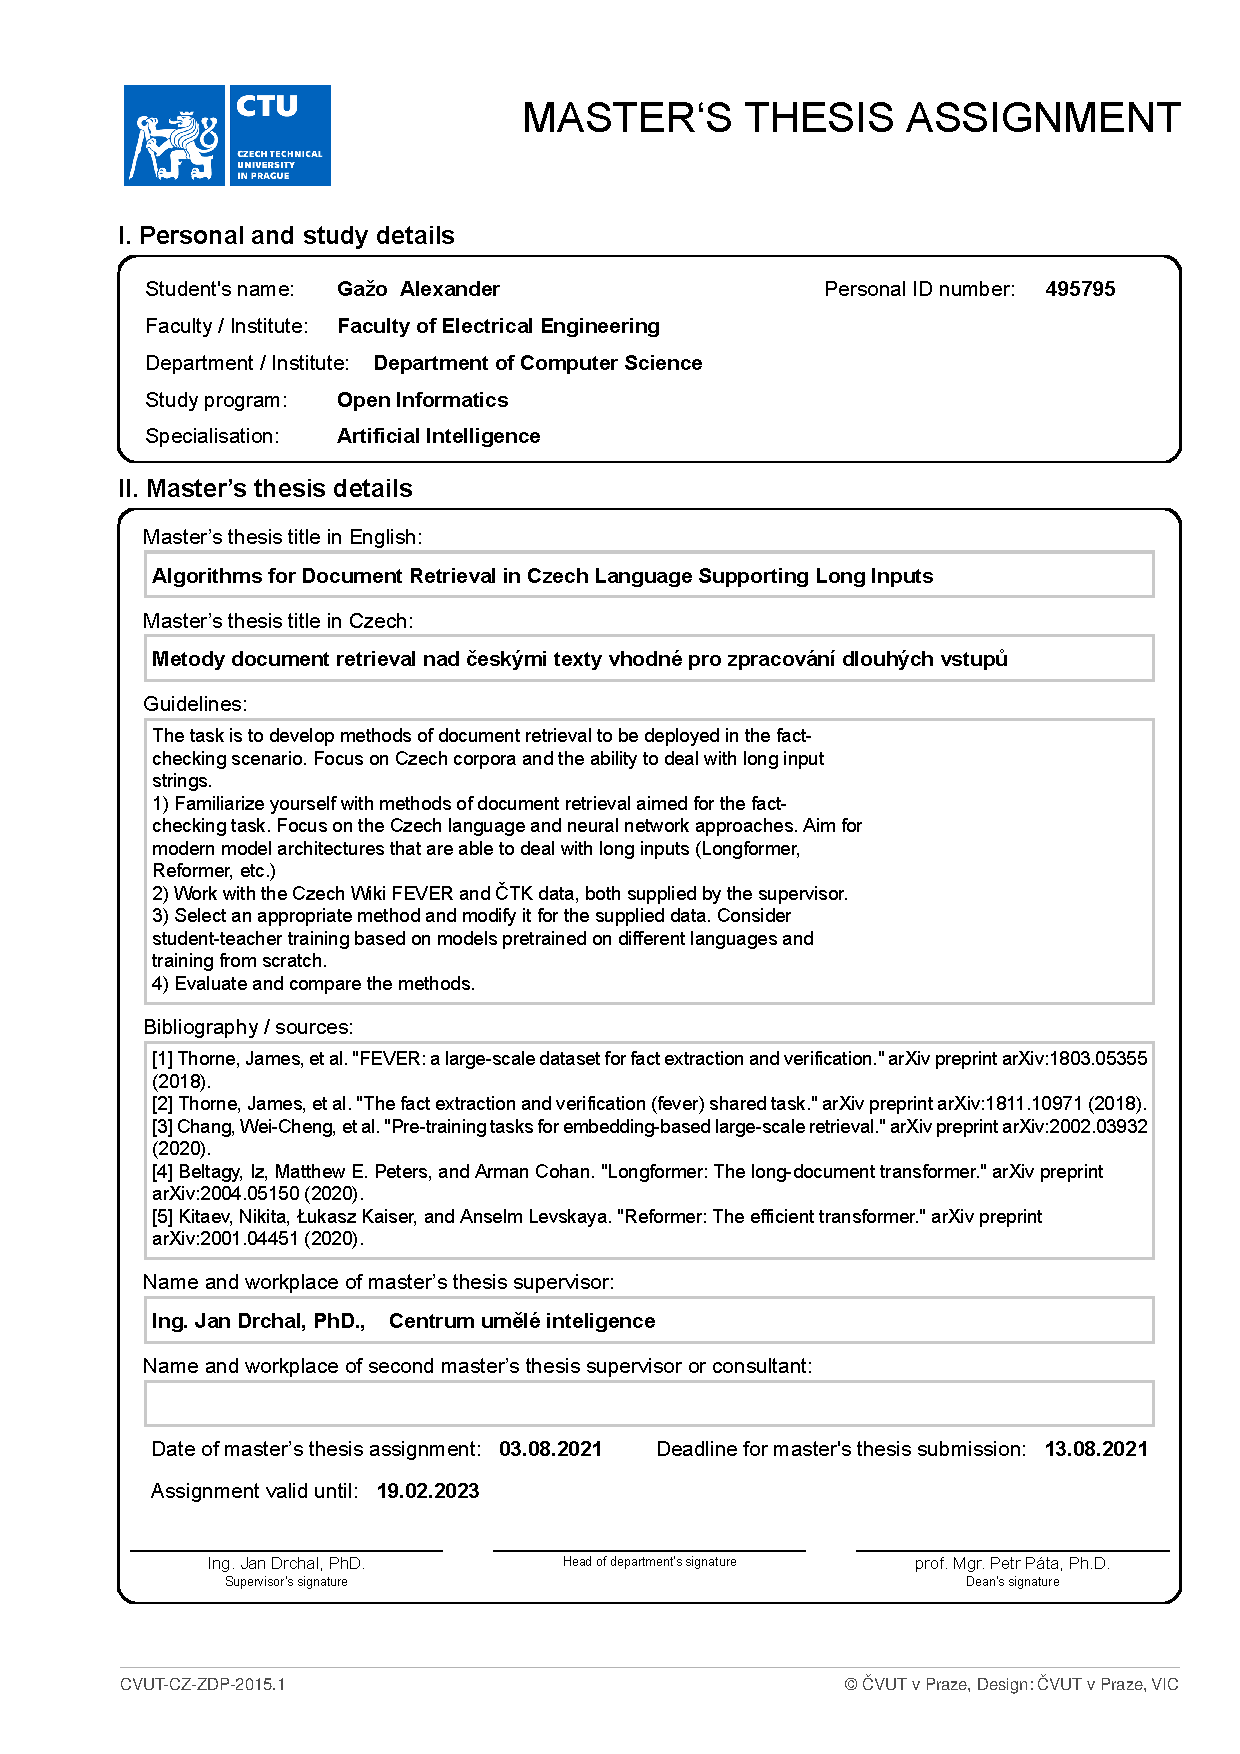
\includepdf[pages=-]{figures/assignment.pdf}
%%% Here should be a bound sheet included -- a signed copy of the "bachelor
%%% thesis assignment". This assignment is NOT a part of the electronic
%%% version of the thesis. DO NOT SCAN.

%%% A page with a solemn declaration to the bachelor thesis

\openright
\hypersetup{pageanchor=true}
\pagestyle{plain}
\pagenumbering{roman}
\vglue 0pt plus 1fill

\noindent
I declare that I carried out this master thesis independently and only with the cited
sources, literature, and other professional sources.

\medskip\noindent\sloppy
I understand that my work relates to the rights and obligations under Act No.~121/2000 Sb., the Copyright Act, as amended.
\vspace{10mm}

\hbox{\hbox to 0.5\hsize{%
In ........ date ............	% FIXME!
\hss}\hbox to 0.5\hsize{%
signature
\hss}}

\vspace{20mm}
\newpage

%%% Dedication

\openright

\noindent
\Dedication

\newpage

%%% Mandatory information page of the thesis

\openright

\vbox to 0.5\vsize{
\setlength\parindent{0mm}
\setlength\parskip{5mm}

Title:
\ThesisTitle

Author:
\ThesisAuthor

\DeptType:
\Department

Supervisor:
\Supervisor, \SupervisorsDepartment

Abstract:
\Abstract

Keywords:
\Keywords

\vss}

\vbox {
\begin{otherlanguage}{slovak}
\setlength\parindent{0mm}
\setlength\parskip{5mm}

Názov práce:
\ThesisTitleSk

Autor:
\ThesisAuthor

\DeptTypeSk:
\DepartmentSk

Vedúci bakalárskej práce:
\Supervisor, \SupervisorsDepartmentSk

Abstrakt:
\AbstractSk

Kľúčové slová:
\KeywordsSk

\end{otherlanguage}
\vss}

\newpage

\openright
\pagestyle{plain}
\pagenumbering{arabic}
\setcounter{page}{1}


%%% A page with the automatically generated table of contents of the bachelor thesis

%\setcounter{tocdepth}{1}
\tableofcontents
\listoffigures
\listoftables

%%% Each chapter is kept in a separate file
\chapter*{Introduction}
\addcontentsline{toc}{chapter}{Introduction}
\section*{Motivation}
At its early stages, the internet was envisioned to become the pinnacle of joint human effort to gather and easily retrieve expert knowledge on virtually any topic.
However, with many laypeople connected to the internet, extensive and aggressive advertising, and adversarial agents such as foreign powers or simply malicious individuals, the information on the internet is becoming harder to be trusted.
The information overload created by these agents results in an ``opaque'' state of the internet, where relevant and accurate information is hard to find in the mass of similarly sounding, non-professionally written sources.
Fact-checking the claims manually, therefore, becomes very expensive and time-consuming - bordering on unfeasible.
Nevertheless, multiple projects focused on fact-checking have emerged. 
Various platforms such as Instagram\footnote{\url{https://about.fb.com/news/2018/05/hard-questions-false-news/}} and Twitter\footnote{\url{https://blog.twitter.com/en_us/topics/product/2021/introducing-birdwatch-a-community-based-approach-to-misinformation}} have incorporated fact-checking mechanisms, mainly on viral post and posts of politicians. 

In Czechia and the Slovak Republic, a popular project is Demagog\footnote{\url{https://demagog.cz}}, whose goal is to verify politicians' claims.
The claim verification is carried out manually using primary sources. 
Similar foreign projects are PolitiFact\footnote{\url{https://www.politifact.com/}}, Factcheck.org\footnote{\url{https://www.factcheck.org/}}, and Washington Post Fact Checker\footnote{\url{https://www.washingtonpost.com/news/fact-checker/}}.
Multiple past "public debates", such as the European migrant crisis or the current coronavirus pandemic, have highlighted the need for such systems since there is a need for accurate and up-to-date information.
The process is very labor-intensive, and thus, there is a natural demand for automatization.

The recent advances in natural language understanding, mainly the introduction of transformer architecture \citep{attention-is-all-you-need} and the BERT model \citep{bert}, led to new research on the use of neural methods in fact-checking.
The FEVER\footnote{\url{https://fever.ai/}} paper \citep{fever} has led this effort since 2018, focusing on creating a dataset meant for training neural models.
They succeeded in creating a sizeable human-annotated dataset and were able to train a pipeline model on it.
The model first retrieved relevant documents (the document retrieval task) and then labeled the initial claim based on these documents. 
%Since then, the FEVER team held multiple shared tasks, and the pipeline approach proved to be adequate.
With better models released every year, the long-term goal is to create a model capable of correctly assessing a claim's truthfulness and provide satisfactory evidence. However, creating helpful tools for journalists to assist them in the fact-checking scenario is the goal for now.

On the other hand, the advances also provide new ways of creating false information on a large scale. Such an example is the recently introduced GPT-3 model \citep{gpt}, which is able to generate human-sounding English texts.
The potential ability of adversaries to flood the internet with fake news articles emphasizes the need for scalable fact-checking tools.

Automatic fact-checking should not be thought of as the miracle cure to the fake news problem, which is much more complex and deserves a society-wide approach.

\section*{AI in Journalism}

This thesis is one of the multiple theses written by the fact-checking team at ČVUT, led by Ing. Jan Drchal, Ph.D., as part of the AI in Journalism project, supported by the Transformation of Journalisms Ethics in the Advent of Artificial Intelligence (TL02000288)\footnote{\url{https://starfos.tacr.cz/cs/project/TL02000288}} grant from the Technology Agency of the Czech Republic.
Our team focuses on creating a Czech fact-checking dataset from the ground up, and developing usable Czech models for the fact-checking task, inspired by FEVER \citep{fever} and \citet{danish_fever}.
The dataset is based on Czech news articles provided in cooperation with the Czech News Agency\footnote{Česká Tlačová Agentúra (ČTK)} -- we refer to the completed dataset as the ČTK dataset. 
Our colleague \citet{ullrich} describes the creation of the ČTK dataset, which consisted of building a Czech annotation platform, working with annotators (students of the Faculty of Social Sciences at Charles University, one of our partners), and analyzing and cleaning up the gathered data.
The works from colleagues \citet{dedkova} and \citet{rypar} deal with various aspects of document retrieval -- the use of hybrid (multi-stage) models and the performance of different embedding paradigms, respectively.

\section*{Transformer Models}

The original transformer architecture \citep{attention-is-all-you-need} and BERT-model \citep{bert} are based on feeding fully-connected feed-forward networks with token representations aggregated from the whole text, meaning that the information from the input tokens (words or subwords) is adjusted according to their whole context. 
This mechanism, named ``attention'' by the authors \citep{first-attention}, introduces quadratic time complexity by ``attending'' to all the input tokens for each input token.
The input of BERT is thus usually limited to 512 tokens as a design choice.
Working with this restriction, we decided to split the \CTK{} articles into paragraphs and perform document retrieval on them, theoretically losing joint article meaning.

In this thesis, we study this practice and compare it to working with full articles using BERT-based models with altered attention mechanisms such as \nystr{} \citep{nystrom}, Longformer \citep{longformer} and Reformer \citep{reformer}.
The changes allow for longer inputs without increasing the computation cost, compromising in other areas.

\section*{Thesis Outline}

This thesis focuses on the document retrieval part of the fact-checking pipeline.
Specifically, it deals with models suitable for processing long Czech documents.

The first chapter deals with fact-checking as a formal task and the past advances in this field.
The next chapter formally defines document retrieval and introduces traditional as well as novel approaches. 
% The datasets created in the project are described in the third chapter, where t
% In Chapter \ref{chap:docret}, we formally define document retrieval, introduce methods that are already in use, and methods that we will be exploring further in this thesis. 
The FEVER dataset, its Czech-translated version, and the ČTK dataset are in-depth described in the third chapter.
We also analyze the length of the documents upon which the datasets are built.
% The before-mentioned datasets are in-depth described in the next chapter (Chapter \ref{chap:data}).
We dedicate the last two chapters to the proposed solutions and the results of the evaluation.

\chapter{Fact-Checking}

\section{Task Description}

We look at fact-checking as a crucial part of journalism as a means of covering important events truthfully. 
The goal is to compare the reported fact or claim to the current state of the world (the knowledge base), or at least its assumed truthful approximation, in our case the corpus of \CTK{} news articles (\CTK{} infobank) and the Czech Wikipedia.
From the comparison, we can ``check'' the truthfulness of the claim -- proclaiming it to be true, false, or unverifiable. 
Thus, we can think of the task of fact-checking as a classification problem with labels True, False, and Not Enough Info (NEI). 
The claims are usually one or a few sentences long strings stating some fact or facts. 
There are platforms, such as Demagog.cz, which also use a category labeled ``misleading'', reserved for facts that are technically true but imply additional, false meaning.
For now, our models do not use this category, although it may be used in further research.

\begin{figure}[h!]
    \centering
    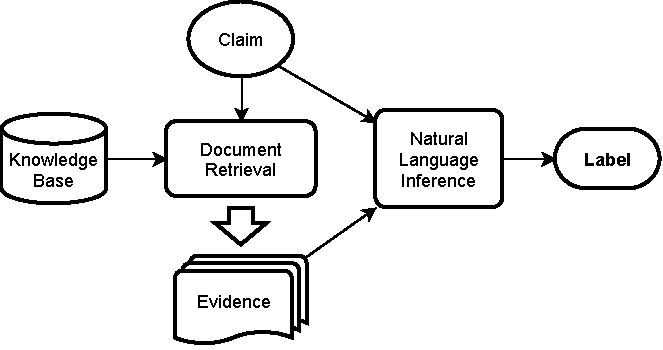
\includegraphics{fc_pipeline_label.pdf}
    \caption[Fact-Checking Pipeline]{Fact-checking pipeline diagram.}
    \label{fig:pipeline}
\end{figure}

To label a claim true or false, we also need to provide evidence validating or refuting the claim.
For our uses, the evidence is one or multiple news articles in \CTK{} infobank (the collection of the articles), which we consider an adequate approximation to the actual world state.
The infobank naturally provides a somewhat distorted image of reality since some world knowledge is already assumed by the journalists, and the original information may be compressed by the article form. 
Therefore, approaches based on language comprehension face the challenge of inferring real-world knowledge from somewhat distorted data. 

The above-described approach can be formulated as a sequence of subtasks (pipeline) depicted in Figure \ref{fig:pipeline}. The first step is to retrieve a collection of relevant documents from the knowledge base. This step is called document retrieval. Then, the Natural Language Inference task is performed, classifying the claim based on the selected sentences.

\section{Related Work}

There exists a number of traditional fact-checking projects such as Demagog\footnote{\url{https://demagog.cz}}, PolitiFact\footnote{\url{https://www.politifact.com/}}, Factcheck.org\footnote{\url{https://www.factcheck.org/}}, and Washington Post Fact Checker\footnote{\url{https://www.washingtonpost.com/news/fact-checker/}}, focus on fact-checking politicians' claims as well as general viral news. 

\begin{figure}[h!]
    \fbox{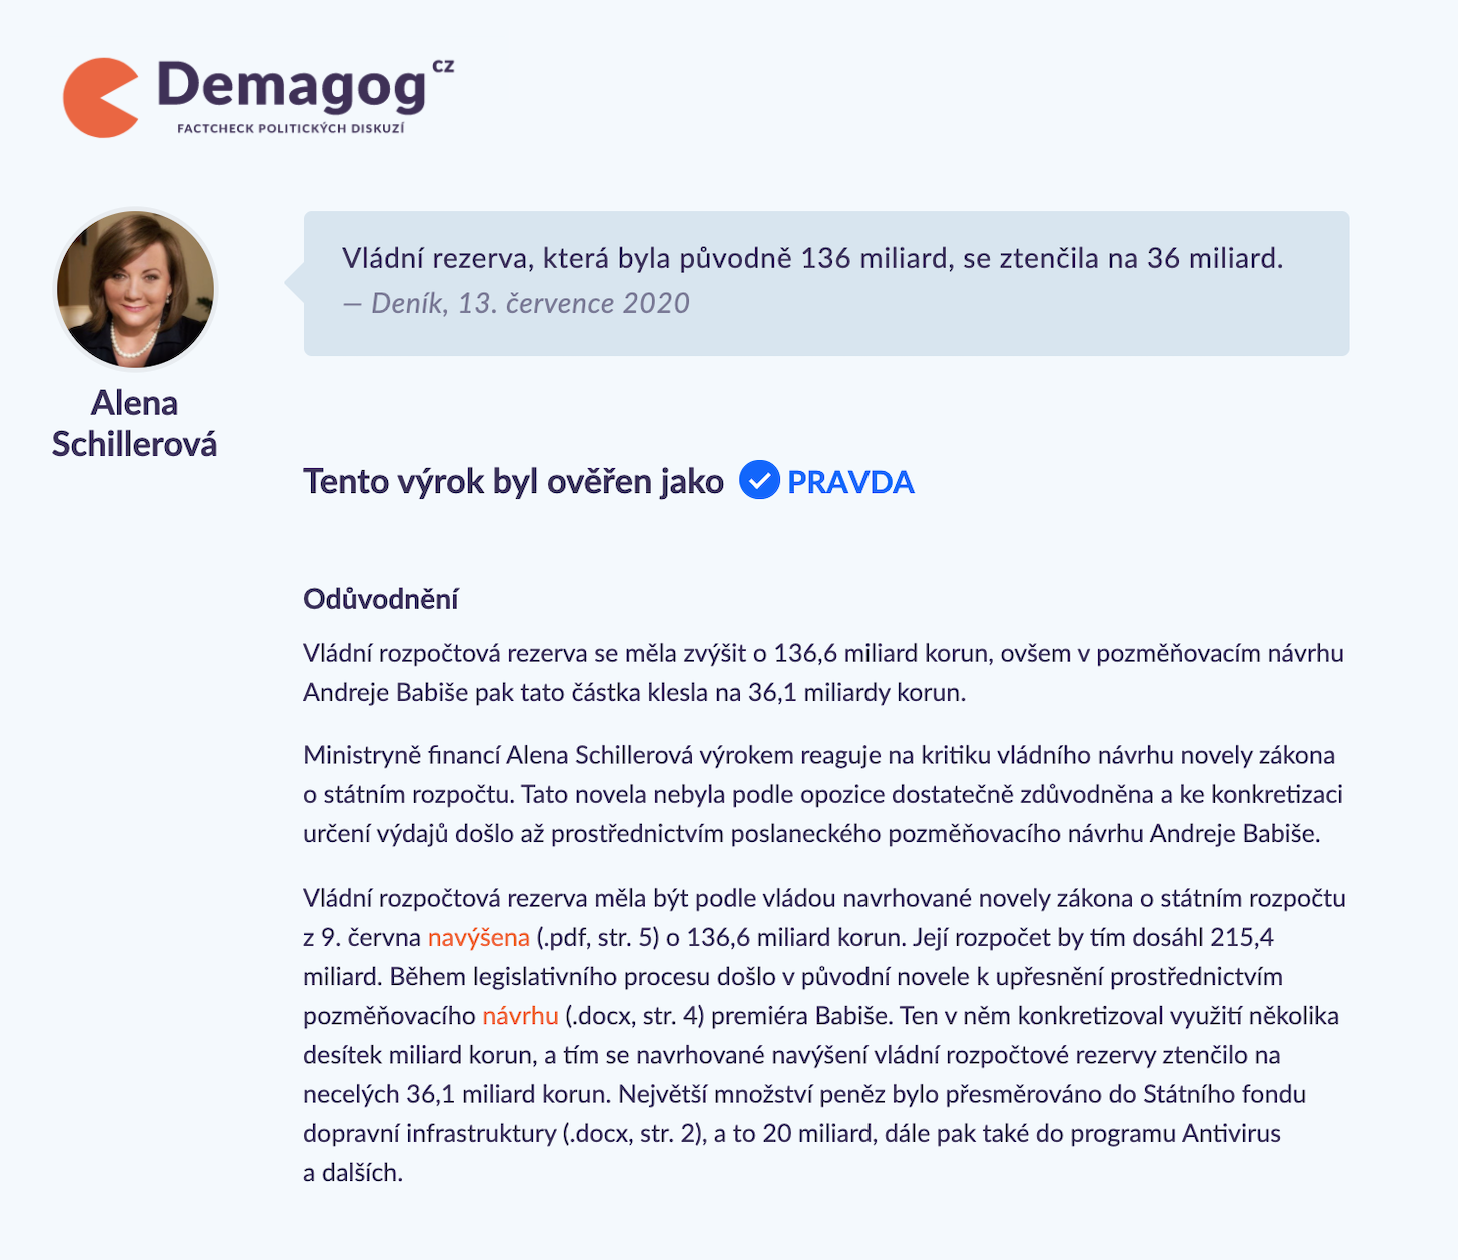
\includegraphics[width=142mm]{demagog.png}}
    \caption[Czech Demagog Entry Example]{Example claim, verdict, and its justification from the Czech Demagog project. Available at permanent address \url{https://demagog.cz/vyrok/19500}.}
\end{figure}

Regarding automatic fact-checking, as of writing this thesis, we are not aware of any other Czech fact-checking datasets other than \citep{czech-fact}.

In the English language, \citet{fever} created the Fact Extraction and Verification (FEVER) dataset; the first large-scale dataset focused on open-domain fact-checking.
The pipeline (Figure \ref{fig:pipeline}) also appears in \citep{fever}, with the addition of the Sentence Selection step, where sentences forming the evidence are extracted after the document retrieval step.

The authors of the FEVER dataset also announced a shared task \citep{fever-2018-shared-task} in which ``The task challenged participants to classify whether human-written factoid claims could be \texttt{SUPPORTED} or \texttt{REFUTED} using evidence retrieved from Wikipedia.'' The results presented in \citep{fever-2018-shared-task} confirmed the pipeline design as the best performing submissions adhered to the design. The authors continue in organizing shared tasks with various modifications, such as \citep{fever-2019-shared-task-adversial} with claims designed to mislead the models and the current task\footnote{\url{https://fever.ai/task.html}(accessed 26th July 2021)} with a focus on an unstructured knowledge base.

%The fact-checking task is similar to the question answering (QA) task in retrieving the evidence. 
% However, QA queries (claims) are often made of very relevant words and thus naturally contain cues for finding relevant documents.

%%%%%%%%%%%%%% DON'T USE THIS PSEUDO-DEEP LOLOTHING %%%%%%%%%%%%%%%%%%
% This creates a perceived weakness that some might criticize, that we still rely on some "outside truth", and cannot decide what is objectively true. 
% Since something can be true only in relation to some other facts (the real state of the world, available news sources, etc.) this criticism lacks substance, but still emphasizes the importance of correclty choosing the knowledge database. 
% In our project, the knowledge database is the \CTK{} infobank. 


\chapter{Document Retrieval}
\label{chap:docret}

The term document retrieval refers to the task of finding relevant information to user queries in a large set of records (documents). 
% Therefore, the document retrieval system operates over a database of records, which for this thesis are described in \ref{chap:data}.
One can think of document retrieval as a search in a vast database of documents. 
In this view, web search services, such as Google, are also a form of document retrieval. 
In this case, the database of documents is all the accessible web pages on the internet.

For our uses, the query is the claim to be fact-checked, and the document database is a collection of relevant documents, which we call knowledge base. 

In this chapter, we define the task of document retrieval and introduce traditional and novel (neural) approaches to solving it.
After describing the traditional word-weighting approaches, we examine crucial concepts behind the used neural models.
We then describe the framework which allows us to use the neural models on the document retrieval task.
We then propose a way of applying the models to the document retrieval task.
TODO -- remove one of the two previous sentences.

\section{Formal Description}
\label{sec:formal_descr_dr}
The task can be formally described \citep{two-tower} using a scoring function (sometimes referred to as ranking function) %article before ranking maybe
\begin{equation}
        f_\mathcal{D}\colon\mathcal{D}\times\mathcal{Q}\rightarrow\R
        \label{eq:formal_descr_dr}
\end{equation}
that maps a document-query pair $(d, q)$ to a score $f(d,q)$. 
Then, typically, the documents in pairs with the highest scores are considered to be the proposed solution to the task. 

As mentioned above, this definition also fits descriptions of a range of other tasks such as open-domain question answering \citep{wiki-retrieval} or recommendation systems.

\section{Approaches to Document Retrieval}

The organizers of the \textbf{T}ext \textbf{Re}trieval \textbf{C}onference (TREC) \citep{trec-2020} classify retrieval methods into three categories (with examples):
\begin{itemize}
        \item Traditional -- TFIDF, BM25
        \item Neural Networks using Language Modeling (NNLM) -- BERT-based
        \item Neural Networks -- others
\end{itemize}
We explore NNLM and traditional approaches, emphasizing the NNLM approach while using the latter as the baseline.
The term ``Neural Networks'' is reserved for methods that use neural networks only in some parts of its implementation (such as word embeddings) and do not rely explicitly on language modeling.
We do not explore such methods in this thesis, and therefore, by neural approach, we refer to the NNLM methods.
While both work on entirely different principles, we will use both to generate an indexed version of the knowledge scope.

This chapter further introduces the most common document retrieval methods and new models with great potential while explaining the main points of the theoretical background.

\section{Traditional Approaches}

Traditional approaches covered are weighting schemes, assigning a query-dependent score to each word in each document in the database.

\subsection{TFIDF}

The traditional approaches are motivated by the intuition that relevant documents will contain the same words as those present in the query. 
Longer documents are at an advantage since there is a higher chance of the relevant words being present, so the term count is often normalized by the number of all terms in the document.
This simple metric is called term frequency (TF). 

TF can be ineffective if some of the terms in the query are very common in the document database.
This issue is resolved by introducing inverse document frequency, which informs how common the term is across all the documents.
The base version of IDF:
\begin{equation}
        \text{idf}(t, D)=\log{\frac{\abs{D}}{\abs{\{d\in D: t\in d\}}}}\ .
\end{equation}

% If we combine these two metrics
Multiplying these two metrics, we get the TFIDF weight of term $t$ in document $d$ in document database $D$:
\begin{equation}
        \text{tfidf}(t,d,D)=\text{tf}(t,d)\cdot\text{idf}(t,D)\ .
\end{equation}

\begin{figure}[!htb]
	\centering
	\begin{minipage}{.5\textwidth}
		\centering
		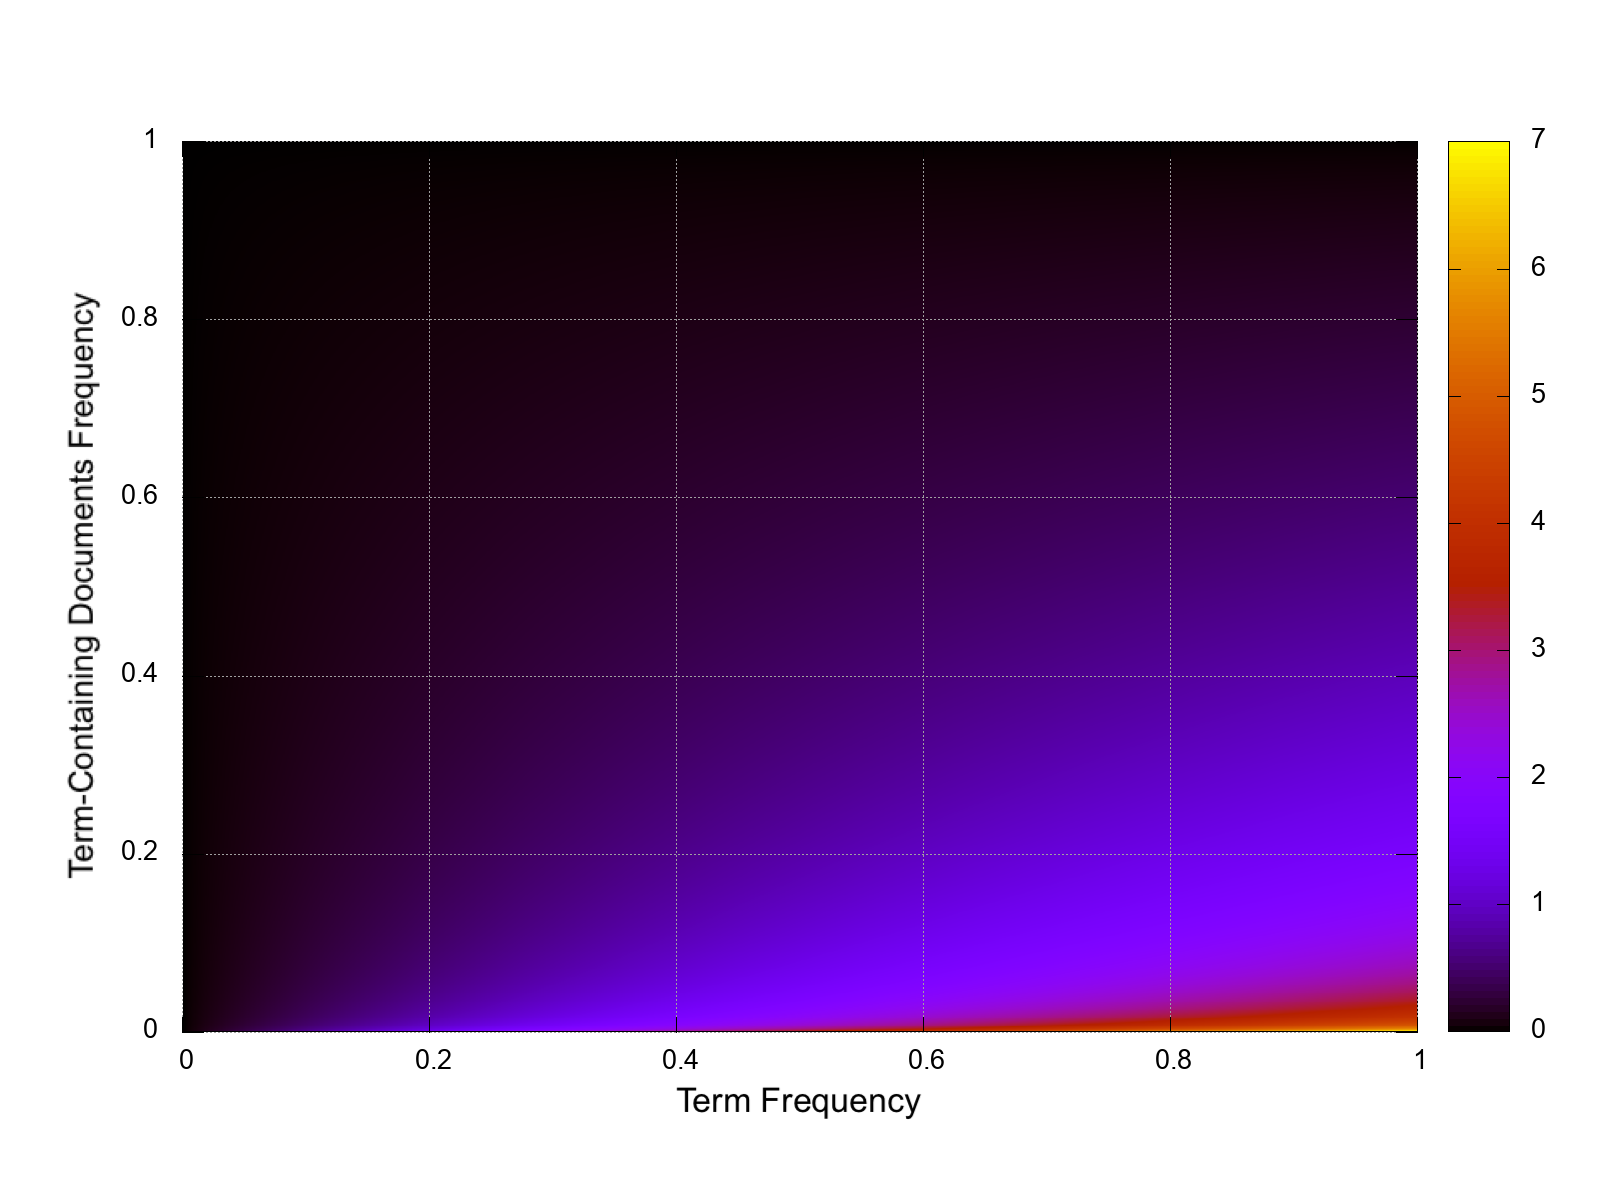
\includegraphics[width=\linewidth]{tfidf_map.png}
	\end{minipage}%
	\begin{minipage}{.5\textwidth}
		\centering
		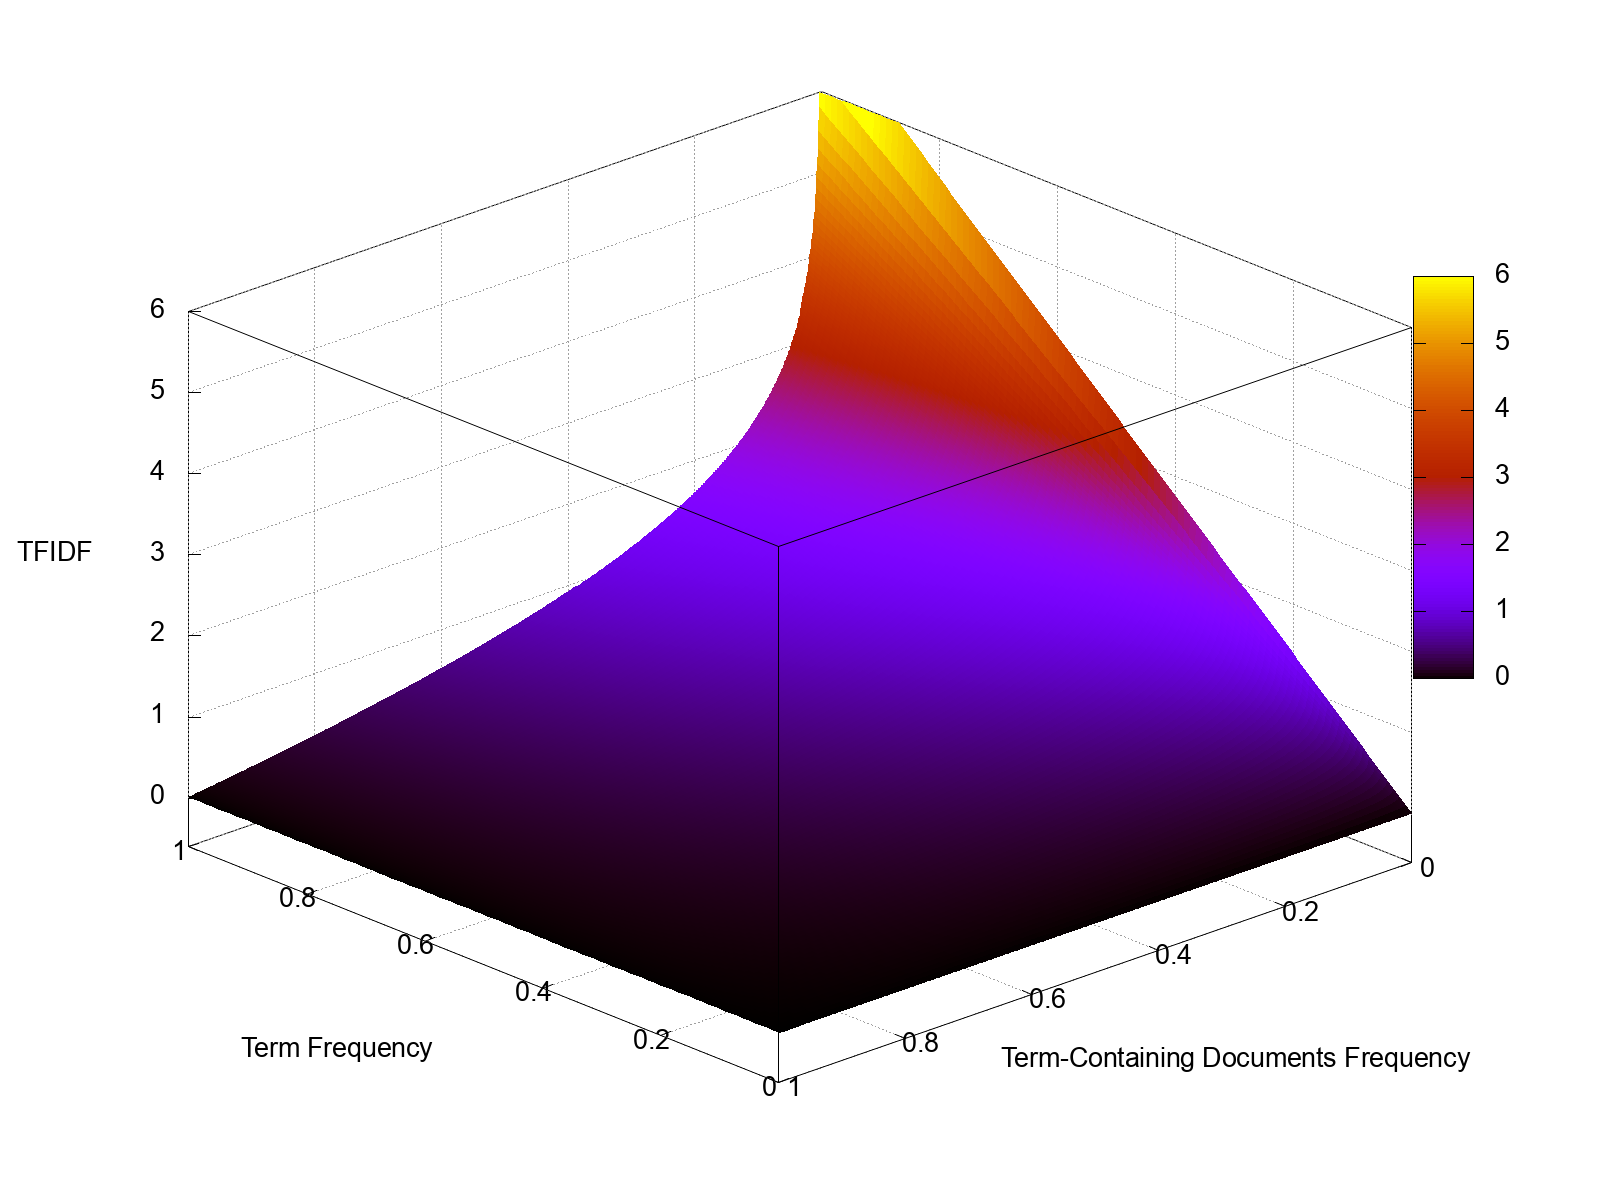
\includegraphics[width=\linewidth]{tfidf.png}
	\end{minipage}
        \caption[Visualization of TFIDF]{Visualization of TFIDF depending on the term frequency and the frequency of the documents containing the term.}
\end{figure}

We have explained how to compute a term's weight (``importance'') for a specific document.
The intuitive formula for query score $f(q, d)$ is then
\begin{equation}
        f_D(q, d)\approx\sum_{t \in q}\text{tfidf}(t, d, D)\ .
\end{equation}
TFIDF is called a weighting scheme precisely for this reason.

Since % term frequency and therefore tfidf is zero when 
$$t\notin d \hspace{1mm}\Rightarrow\hspace{1mm} \text{tf}(t, d) = 0 \hspace{1mm}\Rightarrow\hspace{1mm} \text{tfidf}(t, d, D) = 0\ ,$$
we know that only words in the corpus' vocabulary are important, and thus we can precompute the TFIDF values for each document and word from the corpus' vocabulary.
We obtain $|D|\times {vocabulary\_size}$ matrix $V$ of TFIDF values.
%This formula can be improved -- in this form, it favors longer queries $q$. % DOES IT? TODO
%We can also precompute the TFIDF values for each document and vocabulary word in the corpus.
%Thus we obtain $|D|\times {vocabulary\_size}$ matrix $V$ of TFIDF values.
Here, to simplify length normalization, we normalize the matrix V so that each row has a unit norm.
This step removes the need for normalization in the TFIDF formula, and we may use raw term count instead of the normalized frequency.
To get the relevance of each document to the query $q$, that is $f_D(q, d)$, we first represent the query $q$ as a bag of words vector (BOW), corresponding to the columns of our precomputed TFIDF matrix $V$, ignoring words that appear only in the query.
The resulting score is then the normalized (not to favor long queries) dot product of a row of the matrix and the BOW representation of the query $q$ denoted $\vec{q}$.
We can obtain the scores for every query document pair by matrix multiplication:
\begin{equation}
        f_D(q, d) = \frac{V\vec{q}}{|\vec{q}|} \in \R^{|D|}\ ,
\end{equation}
provided that matrix $V$ is row-normalized (euclidian norm of each row is equal to one).
Please note that this is equivalent to computing the cosine similarity for each document and query vector pair.

This function is one of the first and still widely used \citep{Beel2016} weighting schemes for document retrieval. 

Over the years, multiple versions of the TFIDF approach appeared, differing slightly in formulas or weights of the factors. One of such versions is Best Match 25. %questionable TODO
% maybe put the last sentence as the last sentence of the whole section

\subsection{Best Match 25 (BM25)}

%The following is 
A more complex term weighting scheme is Best Match 25 \citep{bm25}:
%One of the best performing versions \citep{bm_vs_tfidf} is Best Match 25 (BM25) by \cite{bm25}.
%The original formula is:
\begin{equation}
\text{BM25}(q, d) = 
        \sum_{t\in q}
        \text{idf}(t, d)
        \cdot \frac{(k_1 + 1)\cdot\text{c}(t, d)}{k_1(1-b + b \cdot (L_d / L_{avg})) + \text{c}(t, d)} 
        \cdot \frac{(k_3 + 1)\cdot\text{c}(t, q)}{k_3 + \text{c}(t, q)}
\ ,
\end{equation}
where $\text{c}(t,d)$ is the raw count of the term $t$ in the document $d$. $L_d$ and $L_{avg}$ are the current document's length the average document length, respectively.

The first term is IDF.
The second term is TF with two tuning parameters $k_1$ and $b$. Parameter $k_1$ corresponds directly to TF scaling, while parameter $b$ corresponds to scaling by the inverse of the document's length.
The third term follows the same idea as the second term, but the $b$ parameter equivalent is unnecessary since we only have one fixed query.
It shows \citep{schutze2008introduction} that this term is only valid for longer queries $q$, such as whole paragraphs. 
\begin{figure}[h!]
    \centering
    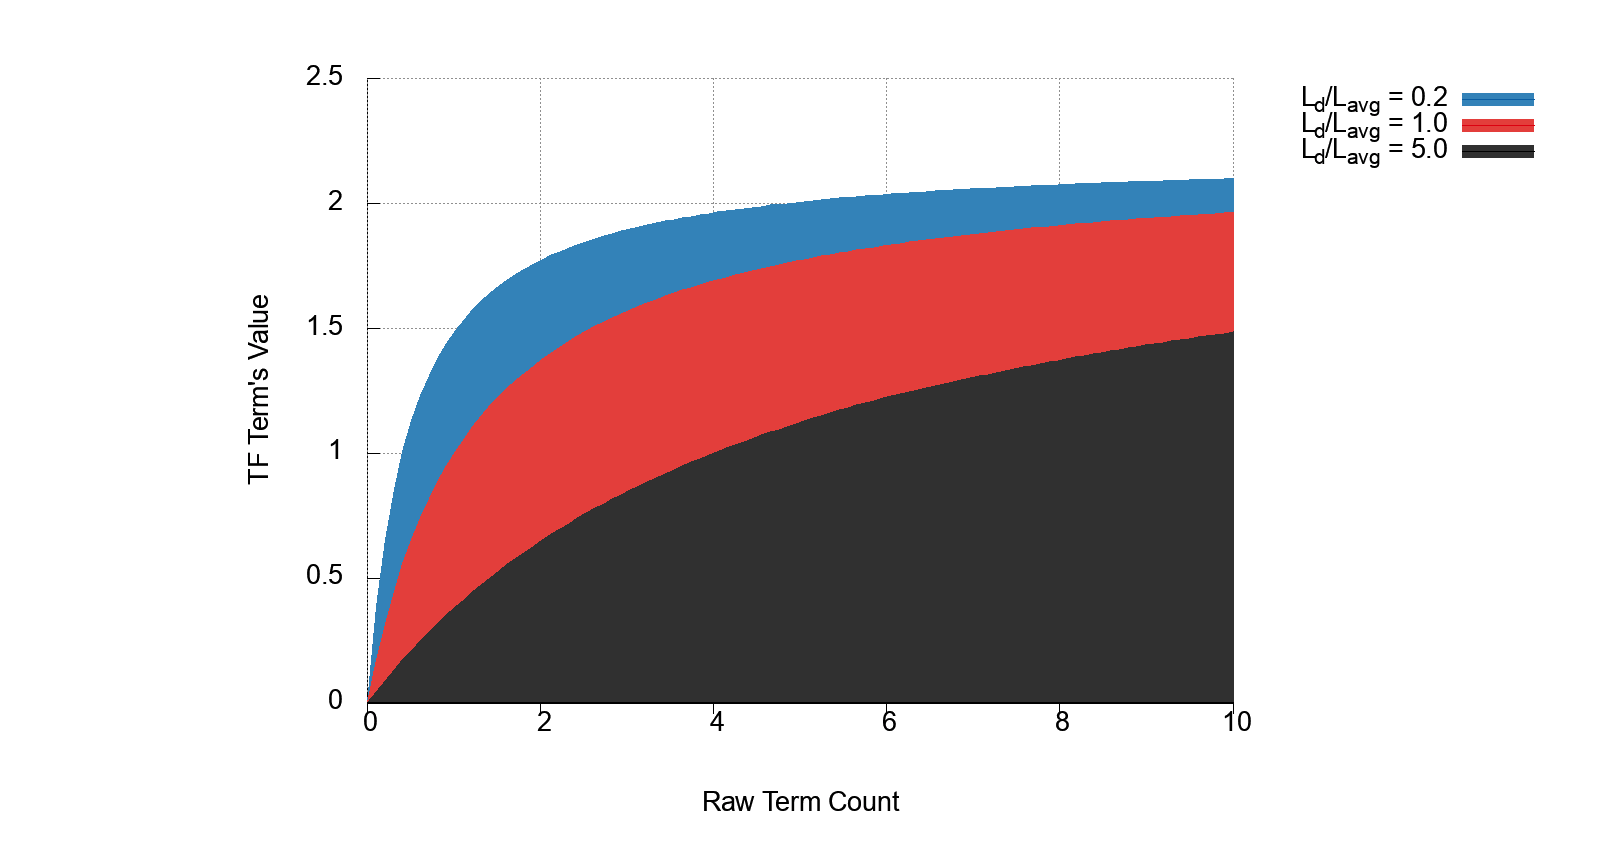
\includegraphics[width=.9\textwidth]{bm25.png}
    \caption[BM25 TF Visualization]{TF term's relation to the length of the current document for $k=1.2$ and $b=0.75$.}
\end{figure}

Since this weighting scheme introduces tunable parameters, it can be trained on data. If the data is not available, \citet[Section 11.4.3]{schutze2008introduction} recommend using $k_1, k_3 \in [1.2;2]$ and $b=0.75$.

%TODO problem with long documents - BM25+ http://sifaka.cs.uiuc.edu/~ylv2/pub/cikm11-lowerbound.pdf

\subsubsection{Final Thoughts}

Some of the apparent disadvantages of traditional approaches are the lack of semantic meaning that comes from the independence on the word order and the exact word matching. % independence???
The former may be improved by using n-grams and the latter using character-level features instead of words, especially in inflected languages such as Czech.
On the other hand, TFIDF is, to this day, a very well-performing low-computation cost ranking function, and as reported by \cite{weak-baselines}, BM25 (if tuned well) is still a solid baseline capable of beating even much more complex neural models.

\section{Neural Approaches}
\label{sec:neural_approaches}

Neural approaches using language modeling are models trained on predicting the correct word given some text before.  % maximizing the likelihood of correct word prediction in a text. 
% More precisely, it is a conditional language modeling since the prediction also depends on provided input.
Recurrent neural network (RNN) architecture was traditionally used for this task.
The RNN was fed encoded tokenized input, returning a hidden state that was next fed into the RNN again along with the next input token's representation.
% The RNN was fed encoded tokenized input, and the RNN predicted the next token as depicted in Figure \ref{fig:lec6_slide23}.
Its hidden states could also be used to encode the input into a fixed-length vector representation, which can be further used to either classify the input or use another RNN (decoder) to generate another sequence.
Intuitively, the vector contains the meaning of the original input. 
Such an approach is the Sequence to Sequence (seq2seq or encoder-decoder) model architecture \citep{seq2seq} with significant use-case in machine translation.

As an improvement to the seq2seq models, the attention mechanism was introduced by \citet{first-attention}.
The authors viewed the RNNs as a bottleneck to improving the model's performance.
They proposed an automatic method of enriching parts of the input with other relevant parts of the input, eliminating the need to process the input as a whole.
The attention mechanism is in-depth described in subsection \ref{subsec:attention}.

% TODO check if this sits nicely
\begin{figure}[b!]
        \centering
        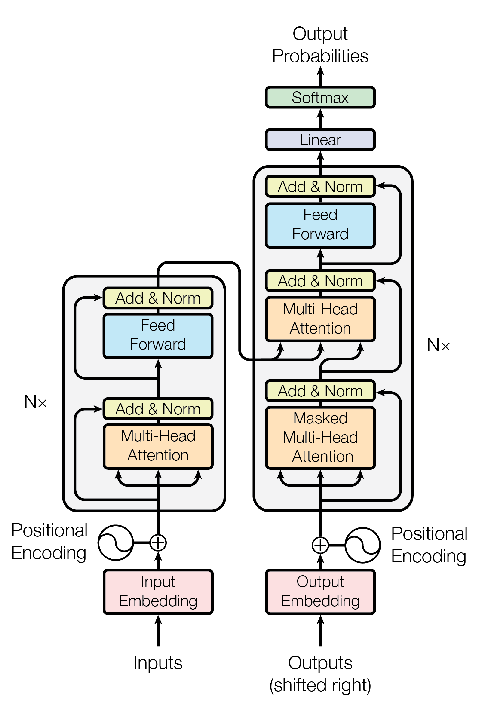
\includegraphics[width=.5\textwidth]{transformer.pdf}
        \caption[Transformer Model Architecture]{The transformer model architecture. Reprinted from \citep{attention-is-all-you-need}.}
        \label{fig:transformer}
\end{figure}

The research paper ``Attention Is All You Need'' by \citet{attention-is-all-you-need} improved the RNN-based seq2seq by introducing the transformer architecture, depicted in Figure \ref{fig:transformer}, by substituting the RNN with multiple ``encoder blocks'', that is, attention layer and feedforward network with skip-connection. 
This resulted in simpler architecture (RNN architectures tend to become very complex when trying to avoid the vanishing gradient problem), parallelization of the computation, and, most importantly, an improved performance. 
The improvement showed that the attention mechanism was crucial to the past achievements of the seq2seq models, hence the paper's name.
%On the other hand, the attention mechanism also introduces quadratic time complexity, which acts as a bottleneck in applications, where a longer input is required.
%That is why the transformer models are generally used with fixed 512 token input length.
%That might be adequate for most applications, but in document retrieval, the documents might get truncated.
%Also, the omission of RNNs meant that the input is not longer sequentially processed. 
%While allowing for parallelization, the position information is lost, and therefore position embedding is added. 
% NAKONIEC SOM TO POUZIL INDE ALE NECHAL AJ TU NECH TO VIEM POROVNAT
% neviem kam to quadratic TODO TODODODODODODOD TOTO ASI CELA DRUHA POLKA FAKT PREC TO SA TAM NEHODI

Then \textbf{B}idirectional \textbf{E}ncoder \textbf{R}epresentations from \textbf{T}ransformers (BERT) \citep{bert} model was introduced. It was ``designed to pre-train deep bidirectional representations from unlabeled text by jointly conditioning on both left and right context in all layers''. 
The model can then be fine-tuned on a specific task using a small amount of labeled data and one additional output layer. 

This was a brief description of how a sequence of research papers -- ``Sequence to Sequence Learning with Neural Networks'' \citep{seq2seq}, ``Neural Machine Translation by Jointly Learning to Align and Translate'' \citep{first-attention}, ``Attention Is All You Need'' \citep{attention-is-all-you-need}, and ``BERT: Pre-training of Deep Bidirectional Transformers for Language Understanding'' \citep{bert} -- led to a shift from RNN-based NLP approaches to, now SOTA, BERT-based approaches.
This research focus is sometimes referred to as BERTology.

In the following sections, we will explain the concepts mentioned above in greater detail.

%The authors trained the model on a large unlabeled corpus using two tasks. 
%The first was to predict random masked words, and the second classified whether the second sentence of two selected sentences immediately follows the first one.
%It is a language modeling encoder capable of non-supervised learning 

\subsection{Word Vectors}

Unlike traditional approaches, neural networks require numbers as their inputs.
Therefore the words (tokens) have to be encoded into a numeric representation with a fixed length.
The word encoding is just another linear layer (with $vocab\_size \times embedding\_dim$ weight matrix), which can be trained from scratch, or one could use pre-trained (for example \citep{glove}) word vectors (the rows of the matrix).

\subsection{Attention Mechanism}
\label{subsec:attention}

The main feature of the transformer models is the attention mechanism. It adjusts each token's embedding based on all the other tokens present in the current input.
This is done by computing three different linear projections of the original input tokens and then, based on certain similarities, combining them back together. 
The attention mechanism is also referred to as self-attention since all the tokens in one input attend to the same input.

The projections are computed using trainable matrices $W_Q$, $W_K$, and $W_V$, producing queries $Q$, keys $K$, and values $V$. Then, we compute the dot product (``similarity'') between the keys and the queries $QK^T$, illustrated in Figure \ref{fig:self-attn}.
The result is normalized by the inverse factor of the square root of the projection dimension. 
Then softmax is applied, and the result is used as the weights for the weighted average of all value vectors. To put it into an equation: 
\begin{equation}
  \text{Attention}(Q,K,V) = \text{softmax}\left(\frac{QK^T}{\sqrt{d}}\right)V\ .
  \label{eq:attention}
\end{equation}
Therefore, for every token, the result is the weighted average of all the value vectors, based on the similarity between the queries and the keys. 
The result is called scaled dot-product attention.

The computation is performed multiple times in parallel with independent projection matrices to make the mechanism more robust.
The results are then concatenated and projected into the final dimensionality.
This extended attention is called multi-head attention.
The intuition is that different heads might learn to attend to different patterns and meaning subspaces.

% TODO check if correct position
\begin{figure}[!htb]
	\centering
	\begin{minipage}{.49\textwidth}
		\centering
		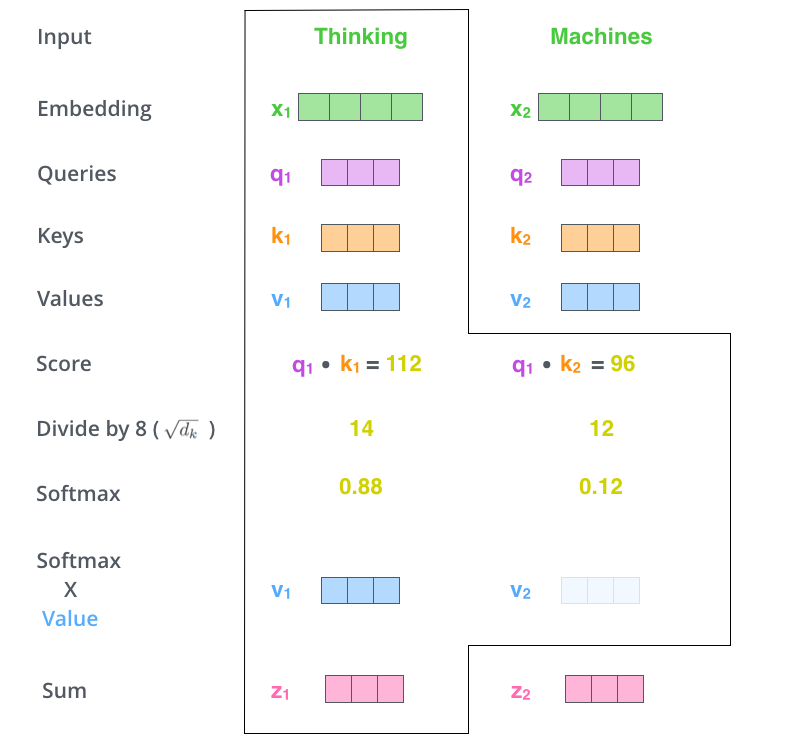
\includegraphics[width=\linewidth]{self_attention_output.png}
                \caption[Attention Mechanism Computation Example]{Example of self attention mechanism with projection dimension 64 and the input ``Thinking Machines''. Reprinted from \citep{illustrated-transformer}.}
	\end{minipage}
        \hfill
	\begin{minipage}{.49\textwidth}
		\centering
		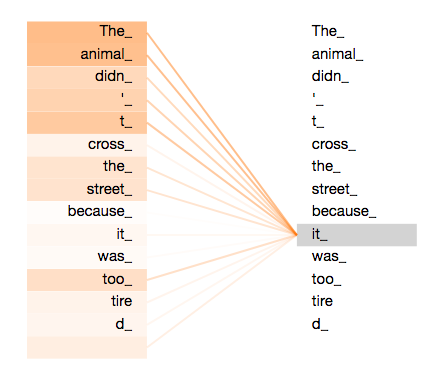
\includegraphics[width=\linewidth]{self_attention_visualization.png}
                \caption[Attention Values Visualization]{Self-attention mechanism example, where the token for the word ``it'' is paying attention to ``the animal'', effectively being substituted for it. The orange color represents the values from $QK^T$. Reprinted from \citep{illustrated-transformer}.}
                \label{fig:self-attn}
	\end{minipage}
\end{figure}

\subsection{Transformer and BERT}

As mentioned earlier, the transformer architecture no longer uses RNNs.
The omission meant that the input is not longer sequentially processed.
While allowing for better performance through parallelization, the position information is lost, and therefore the information has to be added to each input token.
The solution is embedding the position into the same dimension as the word (token) vectors and then adding the positional embedding to the token's embedding.
The position embedding is fixed, non-trainable, and defined as a vector of trigonometric functions applied to the position index, depicted in Figure \ref{fig:pos_emb}.
The authors provide a detailed explanation in \citep[Section 3.5]{attention-is-all-you-need}.

%TODO check position
\begin{figure}[!htb]
        \centering
        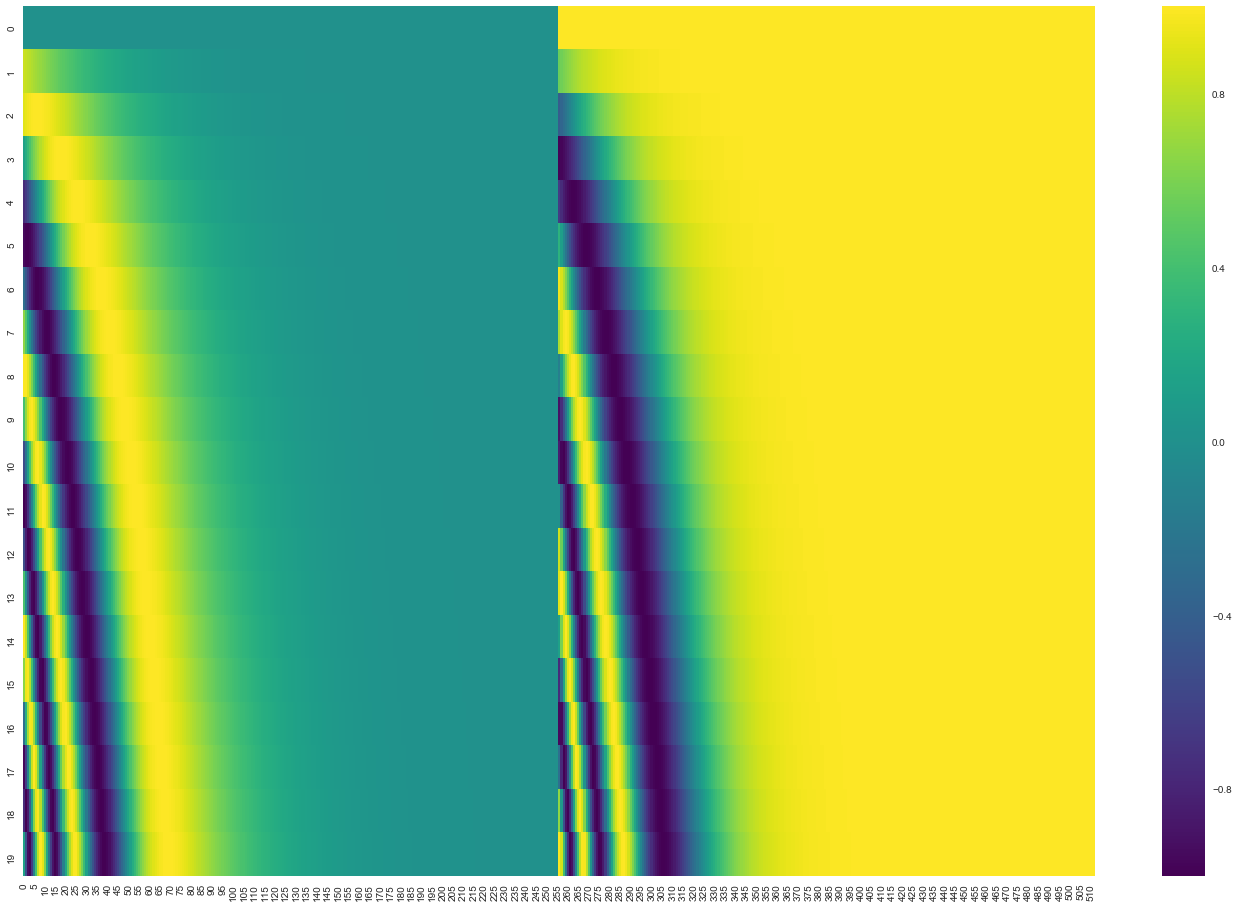
\includegraphics[width=\textwidth]{transformer_positional_encoding.png}
        \caption[Positional Encoding of Transformer's Input]{Transformer positional encoding as described in \citep{attention-is-all-you-need}. Input length is 20 tokens with the embedding dimension of 512. For better visualization, the originally alternating $\sin$ and $\cos$ functions are divided to the left and right half, respectively. Reprinted from \citep{illustrated-transformer}.}
        \label{fig:pos_emb}
\end{figure}

While seq2seq architecture can work with arbitrary sequence types, BERT is a language model working with text input. 
Specifically, it is just the encoder part of the seq2seq architecture, meant for computing real-valued fixed-length vector representation of the input that can further be used by other neural models (usually shallow fully-connected feedforward networks).
The encoder is trained on a large amount of unlabeled text data (corpus) in a phase called pre-training.
This phase, accounting for a great number of the model's parameters ($\approx$ 110 million in its base form), consumes a significant amount of power. 
The model can then be fine-tuned, that is, trained for the task we want to apply it on, such as Named Entity Recognition (NER) \citep{ner}, Natural Language Inference (NLI) \citep{nli-bowman,nli-williams}, or Question Answering (QA) \citep{squad}. 
This is done by usually adding one fully connected layer after the encoder output and relatively short training (of all parameters) with the usage of a smaller amount of labeled data. 

Intuitively, the pre-training ``teaches'' the language and word meanings while the fine-tuning only ``explains'' the final task to the model.

\subsection{Transformer's Computational Limits}

While the benefits of the attention mechanism are undeniable \citep{attention-is-all-you-need}, on the other hand, it introduces quadratic time and space complexity by employing the ``one on one'' approach coupled with the non-linear softmax operation, which prevents various optimization techniques from being applied.
That is why the attention mechanism acts as a bottleneck in applications, where a longer input is required.
Transformer models, therefore, generally have the input length fixed to 512 tokens (shorter inputs are padded, longer truncated).
That might be adequate for most applications, but in document retrieval, valuable information might get lost.

Other parts of the transformer architecture too use a large amount of memory. During training, the activations of every encoder layer have to be stored for back-propagation. Feedforward layers in the encoder blocks are also nontrivially large.

\subsection{BERTology}

The research focus on BERT-like models resulted in many papers introducing minor and major changes to the BERT's architecture.
We will focus on modifying the attention mechanism so that longer inputs are no longer the limiting factor during computation.
%We will focus on the ones modifying the attention mechanism in such a way that larger inputs are no longer the limiting factor during computation. 

\subsubsection{Longformer}

The Longformer architecture \citep{longformer} represents the simplest form of the attention mechanism modification.
Instead of computing the whole $QK^T$, only certain regions (usually specific diagonals) are calculated, thus reducing the model time complexity allowing for longer inputs.

The authors proposed attention windows that ensured that each token attended only to a fixed number of the neighboring tokens. 
Given multiple encoder blocks of the transformer architecture (Figure \ref{fig:transformer}), each token eventually attends to all the input tokens, similarly to CNNs.  
Additionally, a ``dilated'' window attention was used, where the window contains gaps of parametrized size. 
The authors claim that using different sizes of dilation per attention head proved to be beneficial.

In different applications the model performs better with different attention patterns and it might require that some positions attend to the whole input; for example, in question answering, it is essential to attend to the question.
Thus, the authors use another set of projections in the attention mechanism (initialized from the windowed attention) called global attention.
It arises by allowing some positions to attend to the whole input and making the whole input sequence attend to them, as in Figure \ref{fig:longformer_attention}.  %TODO check 

% TODO check position
\begin{figure}[!htb]
        \centering
        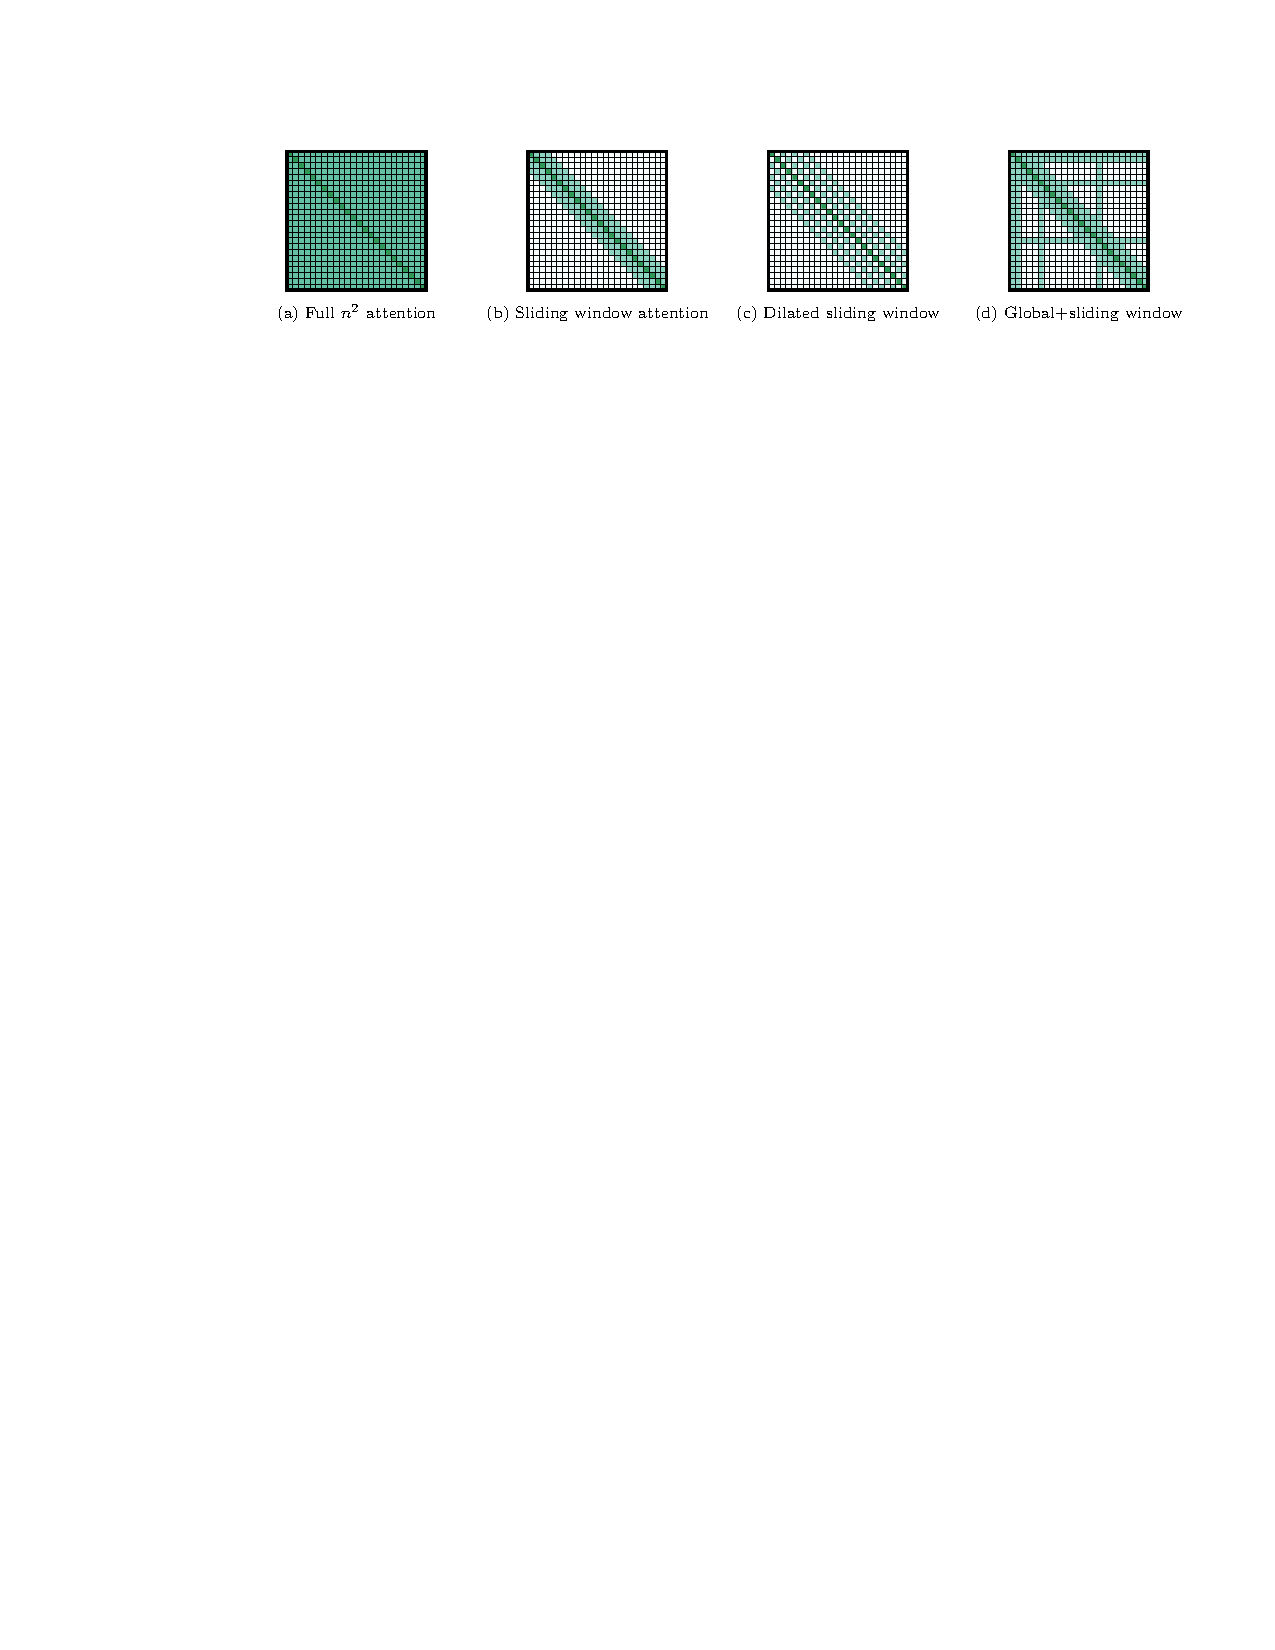
\includegraphics[width=\textwidth]{longformer_attention.pdf}
        \caption[Longformer Attention Patterns]{Original attention and Longormer attention patterns. Reprinted from \citep{longformer}.}
        \label{fig:longformer_attention}
\end{figure}

To utilize the benefits of this sparsified attention, the authors had to implement a custom CUDA kernel capable of computing parts of matrix multiplication effectively.

\subsubsection{BigBird}

The BigBird model \citep{bigbird} adopts a similar approach.
The model also combines windowed and global attention with the addition of random attention.
The random attention pattern is generated per input and in a way to attend to exactly $r$ tokens in one row. Again, the intuition is that thanks to the pattern of the attention matrix, the omitted parts are reachable in just a few layers deep.

The authors prove theoretical guarantees for the model, namely that the attention pattern is able to approximate an arbitrary attention matrix.
However, in the worst case, the number of layers needed is $m$, making the guarantee nonetheless rely on empirical evidence.

\begin{figure}[!htb]
        \centering
        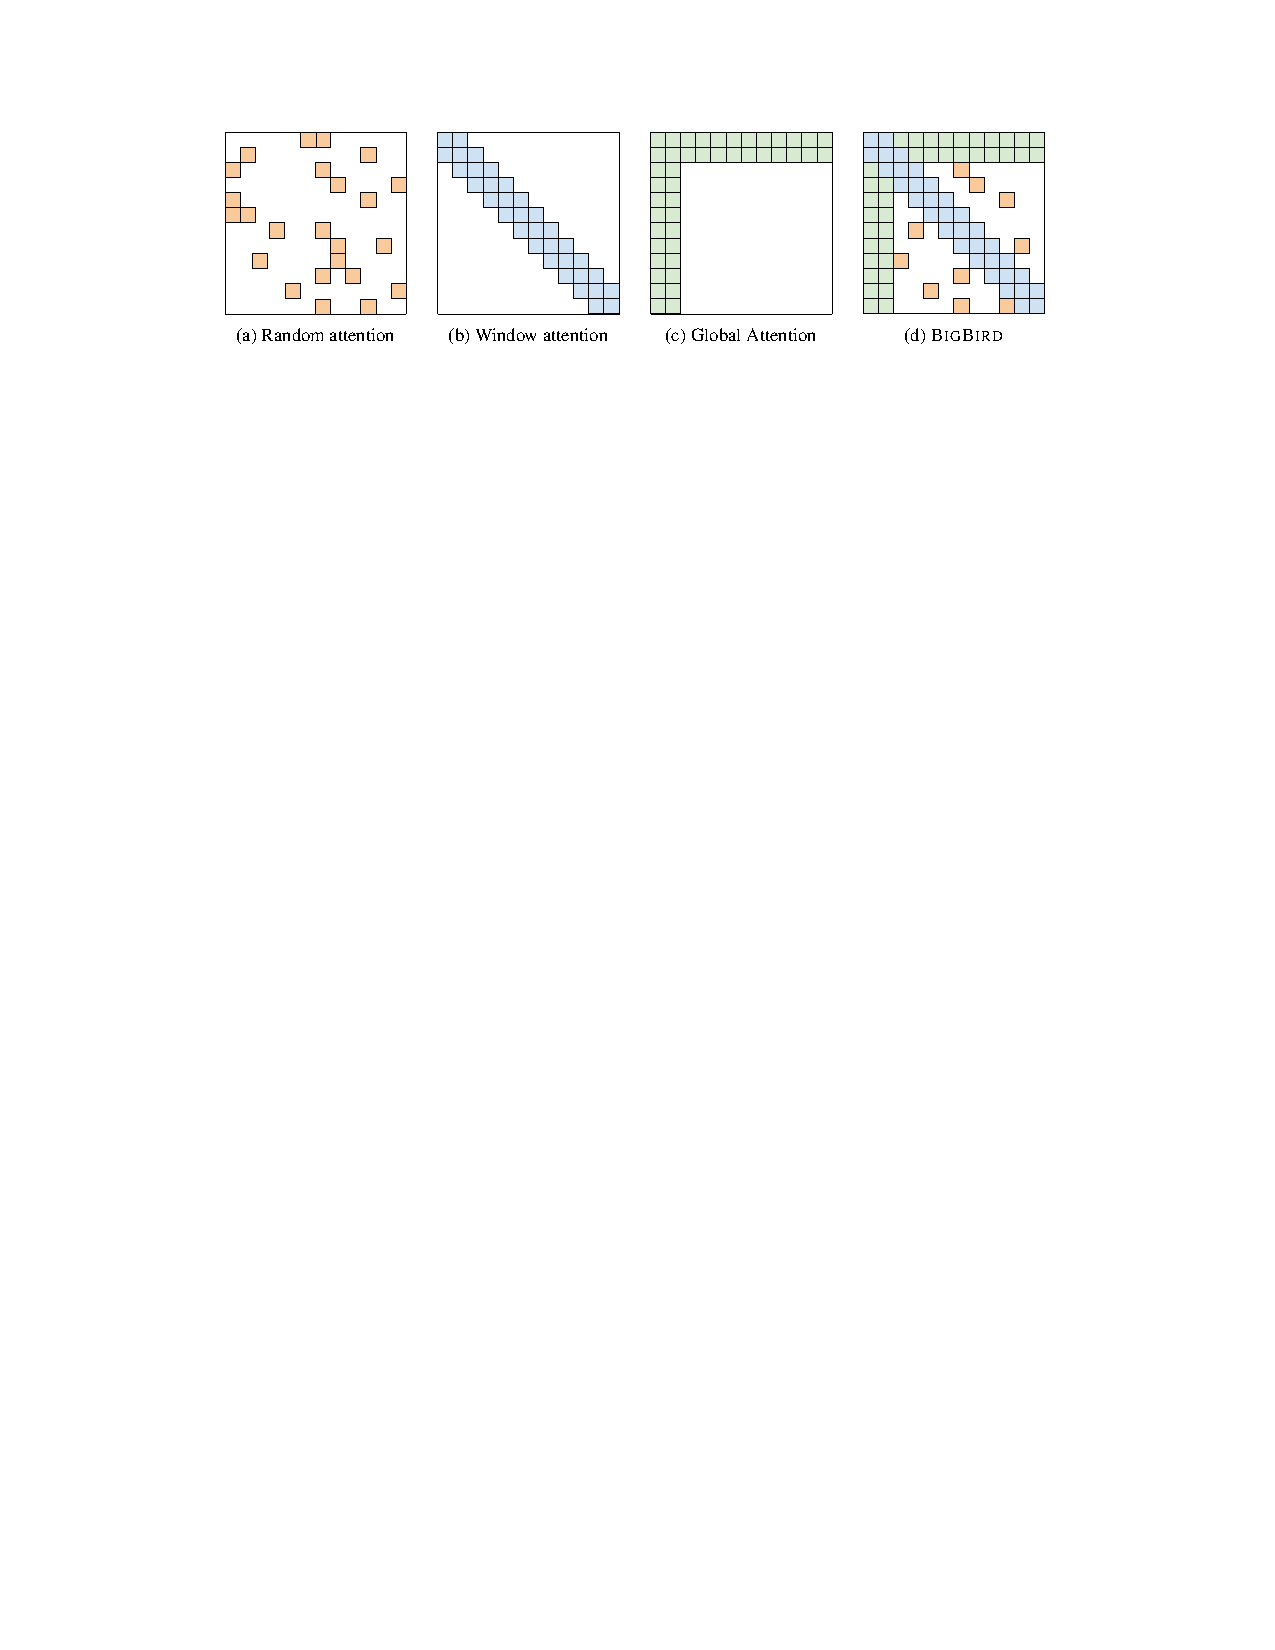
\includegraphics[width=\textwidth]{bigbird_attention.pdf}
        \caption[BigBird Attention Patterns]{BigBird attention patterns with parameters $r=2, w=3, g=2$, the last being the number of first tokens to attend to globally. Reprinted from \citep{bigbird}.}
        \label{fig:bigbird_attention}
\end{figure}

BigBird and Longformer both propose pattern-based attention, granting them $\bigO(n)$ complexity.
However, they do introduce additional meta-parameters, which in order for the model to function perform on BERT's level, have to be set to large values. 

The paper also discusses techniques to make the computation of the patterns suitable for GPU, such as block-attention, where sparse tokens are ``enlarged'' to bigger blocks, and reshaping the final matrix to a rectangle shape.

\subsubsection{Reformer}

Reformer architecture \citep{reformer} offers two changes to the transformer model.
The first is the usage of locality-sensitive hashing (LSH) \citep{lsh} in the attention mechanism, and the second is the use of reversible residual networks (RevNets) \citep{revnets}.

The main idea behind the Reformer's attention is that softmax output from Equation \ref{eq:attention} is influenced most by the largest values of $QK^T$. 
Since the output of $QK^T$ represents the dot products between the rows of $Q$ and $K$, the largest values are those, for which are the vectors from $Q$ and $K$ closest to each other.
The problem of finding the closest vectors is still in $\bigO(n^2)$ since we need to compute the cosine distance between all the vector pairs -- we would need to compute $QK^T$ nonetheless. %??? TODO check grammar
Here the authors utilize LSH for finding the closest vectors.
Hash function $h(x)$ is locality-sensitive if it maps nearby vectors to the same hash with high probability. 
The simplified base idea is that under random linear projections (randomly initialized matrix) into $n_{buckets}$ dimensional space, nearby vectors preserve their orientation, thus sharing the dimension index where they show the highest values.
Multiple random linear projections are performed in parallel to reduce the probability of similar vectors differing in the maximal indices.
After the LSH computation is finished, each vector has been assigned to a ``bucket''.
Then the matrix $Q$ is sorted so that vectors from the same buckets are in a sequence.
What follows is the computation of full attention, but only on parts of the sorted matrix.
The parts are selected so that each bucket attends to all of the vectors in the bucket and one previous bucket, see Figure \ref{fig:reformer_buckets}.
LSH does reduce attention computation time, but it introduces a large constant $c=n_{buckets}^2$ to the memory and time complexity since $n_buckets$ is typically 128.
The authors also noted that setting $Q=K$ did not negatively impact the model's performance, and therefore LSH is applied only to the matrix $Q$.

Another way to look at the LSH bucketing is to compute the dot product of the input vectors with a sequence of $\dfrac{n_{buckets}}{2}$ random vectors followed by their negative counterparts of the same dimension as the input vectors.
Since cosine-similar vectors produce the highest values of dot products, we can be confident that vectors are similar if they shared the highest dot product values with the same random vectors even after multiple rounds of these projections.

\begin{figure}[!htb]
        \centering
        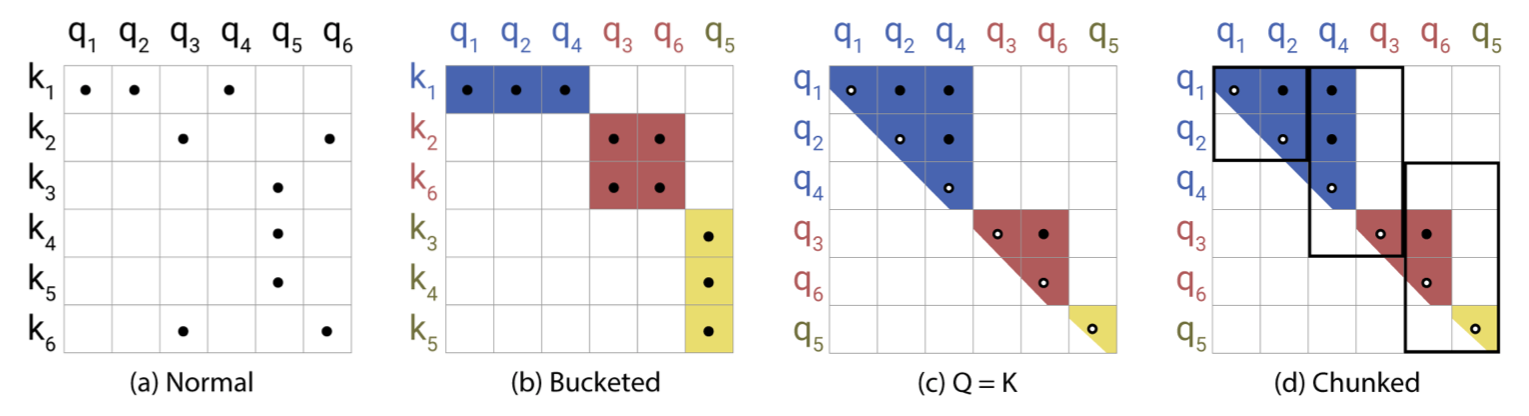
\includegraphics[width=\textwidth]{reformer_buckets.png}
        \caption[Reformer Attention Visualization]{Reformer attention buckets. Reprinted from \citep{reformer}.}
        \label{fig:reformer_buckets}
\end{figure}

In order to reduce the memory complexity, the Reformer model applies three methods.
The first one is the use of RevNets \citep{revnets} discarding the need for storing layers' activations (Figure \ref{fig:revnets}). The second one is the use of ``chunking'' -- feeding only ``chunks'' of input at a time through the linear layers.
The last one is the swapping of the parameters of the currently unused layer from GPU to CPU. This would not be efficient in normal transformers, but since Reformer is able to work with inputs even 64,000 tokens long, the authors claim that ``the amount of compute done with the parameters amortizes the cost of their transfer.''

\begin{figure}[!htb]
        \centering
        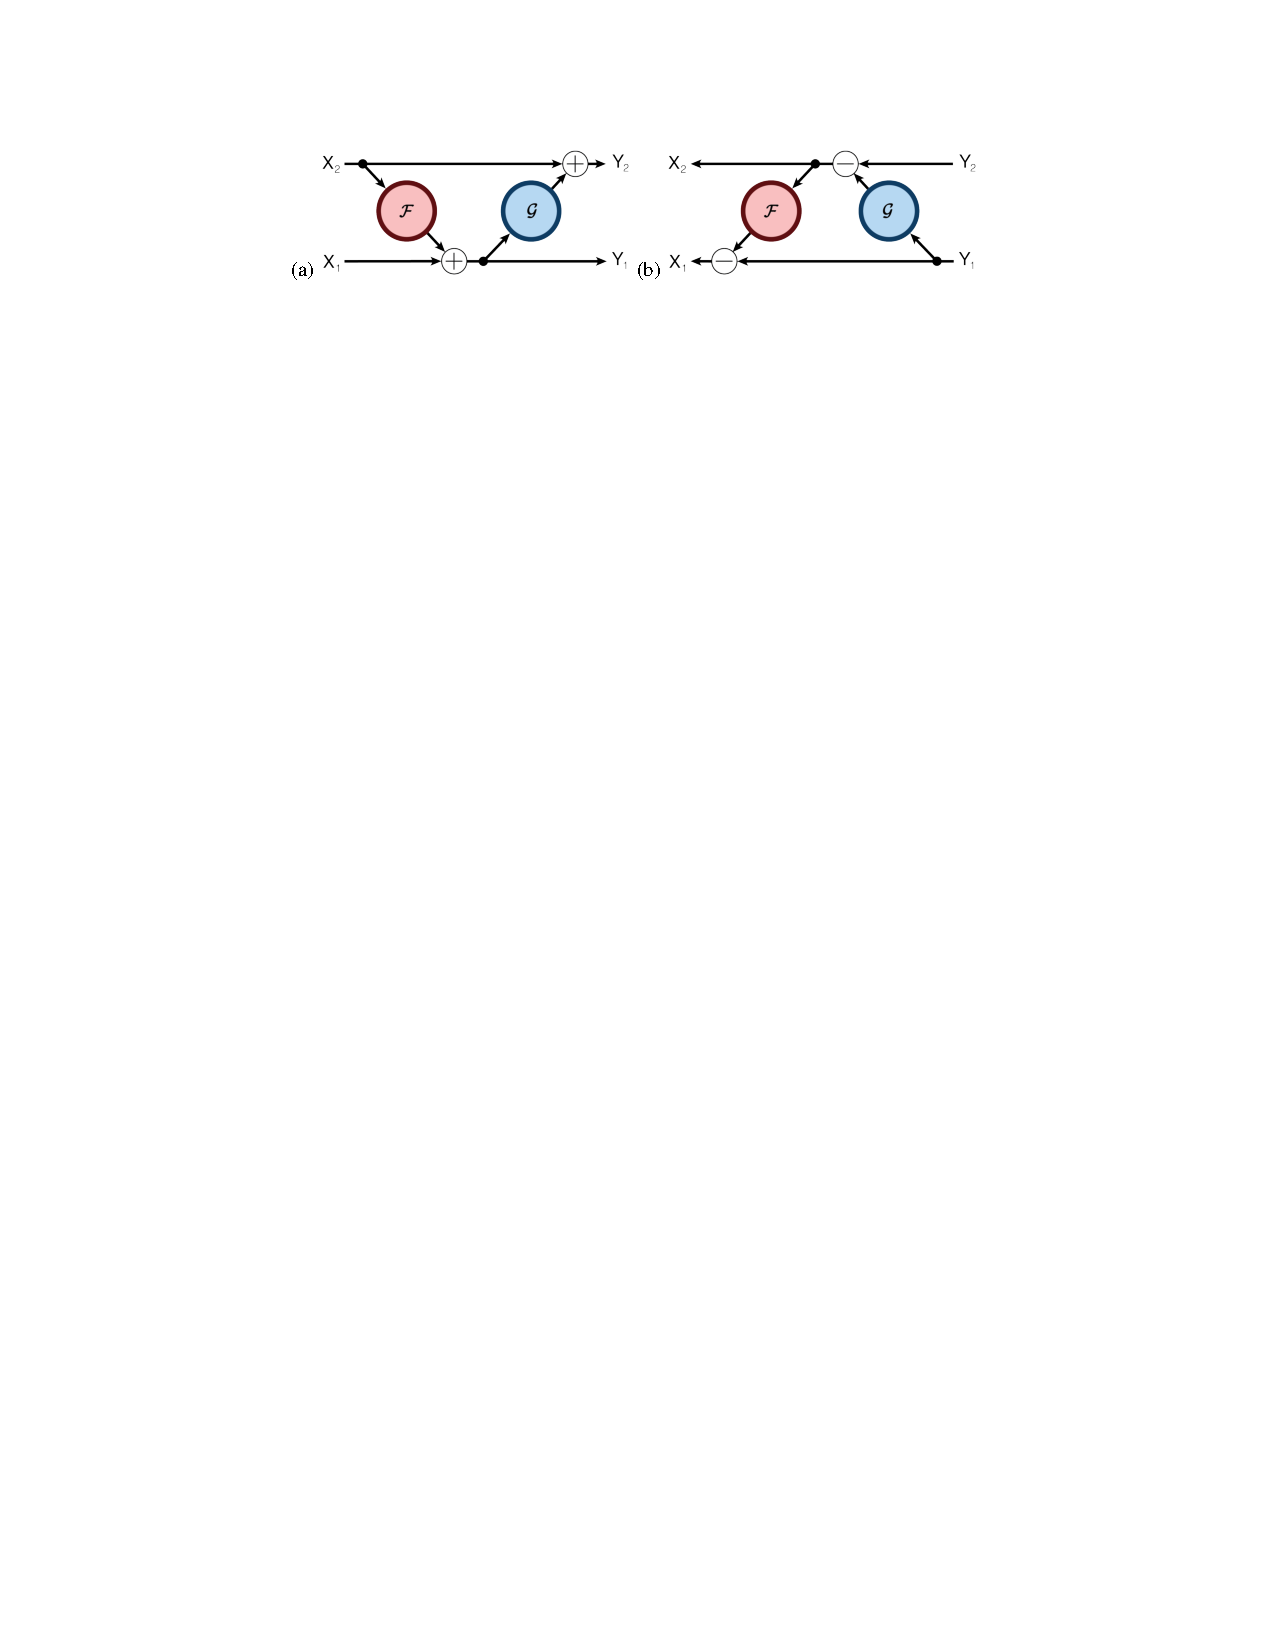
\includegraphics{revnets.pdf}
        \caption[RevNet Scheme]{The forward \textbf{(a)} and the backward \textbf{(b)} computations scheme of a residual block. Reprinted from \citep{revnets}.}
        \label{fig:revnets}
\end{figure}

\subsubsection{Linformer}

Linformer model \citep{linformer} proposes a projection method to make the attention mechanism linear.
The authors propose that the softmax part of the attention is low-rank, and therefore it is possible to perform an approximate calculation in lower dimensions. The theory stands on the distributional
Johnson–Lindenstrauss lemma \citep{JL-lemma}, using its formulation from \citep{JL-formulation}. 
It states that given $k\leq n$, a random gaussian projection from an $n$-dimensional space into $k$-dimensional space with zero-mean and $\frac{1}{k}$ standard deviation, preserves vectors' lengths and pairwise dot products with high probability.
They prove that for the softmax part, the projection dimension $k$ can be set to $\min\{\Theta(9d\log(d)/\epsilon^2),5\Theta(\log(n)/\epsilon^2)\}$ while keeping the approximation error reasonably low \citep[Theorem 2]{linformer}.

The projection matrices $E, F$ are in the proof defined as $E=\delta R, F=e^{-\delta}R$ for $R\in\R^{k\times n}$ with iid entries from $\mathcal{N}(0,\frac{1}{k})$ and a small constant $\delta$.
The attention mechanism itself is changed only by introducing non-trainable projection matrices when computing the keys and the values:
\begin{equation}
        \text{LinAttn}(Q,K,V)=\text{Attention}(Q,EK,FV)=
        \text{softmax}\left(\frac{Q(EK)^T}{\sqrt{d}}\right)FV
        \ .
\end{equation}
The resulting time and space complexity is $\bigO(kn)$. 

The authors also tested multiple techniques of sharing the projection matrices, concluding that the model's results were preserved when all the attention heads and layers used the same $E,F$ matrices, even when $E=F$.
They also proposed using different projected dimensions $k$ for different heads and layers, motivated by Figure \ref{fig:linformer_lowrank} (right), although no tests were performed.

\begin{figure}[!htb]
        \centering
        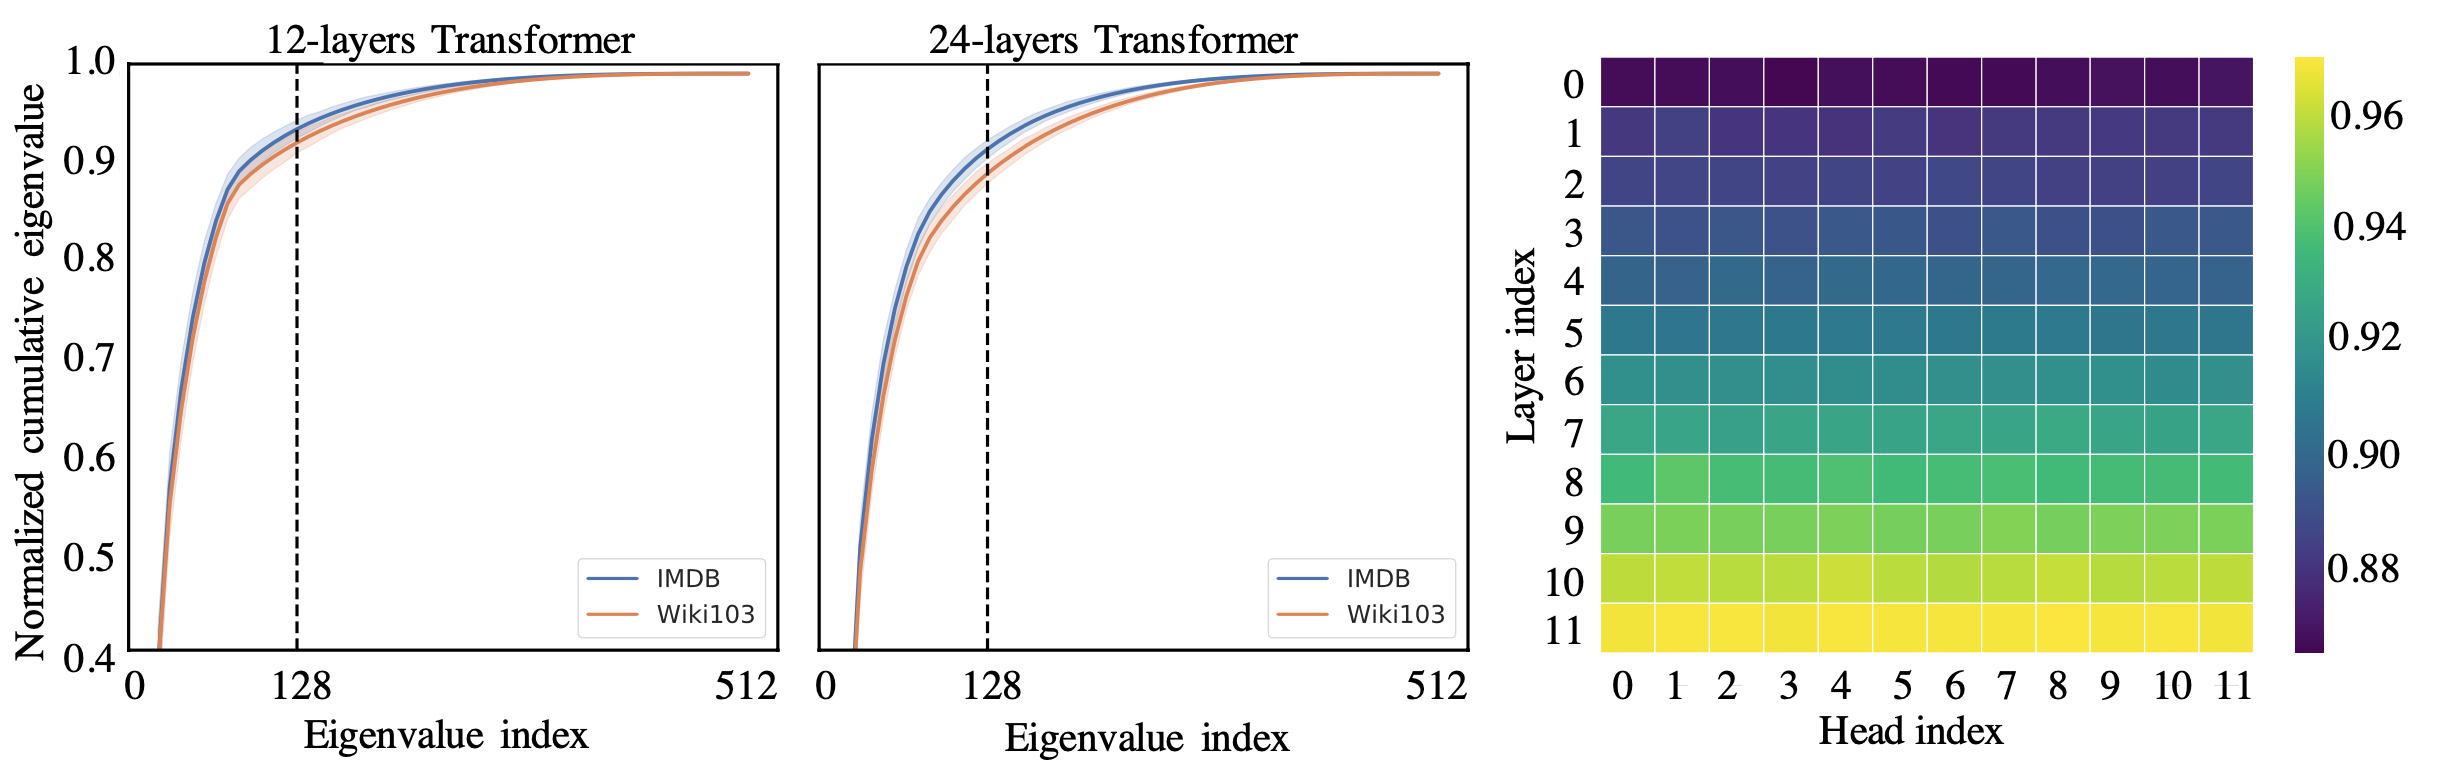
\includegraphics[width=\textwidth]{linformer_lowrank.png}
        \caption[Rank of the Attention Mechanism]{Anecdotal evidence of the low rank of a pretrained transformer's attention mechanism. Higher cumulative sum of eigenvalues indicates the amount of information in the included indices. Reprinted from \citep{linformer}.}
        \label{fig:linformer_lowrank}
\end{figure}

We want to note that \citep[Theorem 1]{linformer} provides no insight since it holds for arbitrary matrix $P$. 
However, the authors do provide anecdotal evidence of the
attention mechanism’s low rank (see Figure \ref{fig:linformer_lowrank}).

\subsubsection{Performer}

Performer model \citep{performer} looks at the self-attention mechanism, concretely at the softmax substep $A=\exp(\frac{QK^T}{\sqrt{d}})$, as a randomized kernel function: 
\begin{equation}
    A_{i,j}=K(q_i,k_j)=\mathbb{E}[\phi(q_i)^T\phi(k_j)]\ ,
\end{equation}
where K is a kernel function $K\colon\R^d\times\R^d\rightarrow\R$ defined for a feature map $\phi\colon\R^d\rightarrow\R^r$.
The authors approximate the attention by using the randomized feature map to define matrices $Q', K'\in\R^{n\times r}$, with the rows equal to $\phi(q_i^T)^T$ and $\phi(k_i^T)^T$, respectively.
Then, by calculating in the parenthesized order
\begin{equation}
        AV = (Q'(K'V))
\end{equation}
the authors reduce the time complexity from $\bigO(n^2d)$ to $\bigO(nrd)$.
The paper then deals with finding suitable randomized feature maps with adequate theoretical assurances. 
The authors propose a general form
\begin{equation}
        \phi(x)=\frac{h(x)}{\sqrt{m}}(f_1(\omega_1^Tx),\dots,f_1(\omega_m^Tx),
        \dots,f_l(\omega_1^Tx),\dots,f_l(\omega_m^Tx))\ ,
\end{equation}
where $f_1,\dots,f_l\colon\R\rightarrow\R$, $g\colon\R^d\rightarrow\R$ and $\omega_1,\dots,\omega_m\overset{\text{iid}}{\sim}\mathcal{D}$ for some distribution $\mathcal{D}\in\powerset{\R}^d$.

The authors conclude their theoretical research by guaranteeing ``unbiased or nearly-unbiased estimation of the attention matrix, uniform convergence and low estimation variance'' for $h(x)=\exp(\frac{||x||}{2})$, $l=2$, $f_1=\cos$, $f_2=\sin$, $\mathcal{D}=\mathcal{N}(0,\textbf{I}_d)$, and ensuring that $\omega_1,\dots,\omega_m$ are perpendicular to each other, \citep[Theorem 4]{performer}.
The parameter $m$ does depend on the L2-norm of the queries and keys, the dimensionality of the embeddings, and the required precision, but does not depend on the input sequence length $n$.

\subsubsection{\nystr{}}

Nystr\"omformer's \citep{nystrom} base idea is to approximate the attention computation by subsampling the original $Q$ and $K$ matrices and using a Nystr\"om-based method \citep{nystrom-matrix-approx} to approximate the full attention. 
The subsampling is done by splitting the $Q$ and $K$ matrices into equally sized segments and then averaging each part into single vectors, calling them landmarks.

The full attention matrix can be written as
\begin{equation}
        \text{Attention}(Q,K,V)=\text{softmax}\left(\frac{QK^T}{\sqrt{d}}\right)V=
        \begin{bmatrix}
                A_S && B_S \\
                F_S && C_S
        \end{bmatrix}V\ ,
\end{equation}
where $A_S\in\R^{m\times m}$ and other matrices are of appropriate shapes, with $m$ being the number of samples (landmarks). 
The authors note that using \citep{nystrom-matrix-approx}, one could approximate the attention by expressing the matrix $C_S$ using the other matrices: $C_S=F_SA_S^\dagger B_S$. The $\dagger$ sign indicates the Moore-Penrose inverse.

Such usage of the Nystr\"om approximation will not help, as the samples can only be obtained after the attention matrix is computed -- the softmax operation needs the whole matrix $QK^T$ (or at least its rows) to be complete. 
Nevertheless, the authors do compute softmax over only the subsampled parts of the $QK^T$ matrix and use the resulting softmax-ed matrices to compute the approximated attention.
The final approximated attention is obtained by 
\begin{equation}
        \widehat{\text{Attn}}(Q,K,V)=
        \left(
        \text{softmax}\left(\frac{Q\tilde{K}^T}{\sqrt{d}}\right)
        \text{softmax}\left(\frac{\tilde{Q}\tilde{K}^T}{\sqrt{d}}\right)^\dagger
        \right)
        \left(
        \text{softmax}\left(\frac{\tilde{Q}K^T}{\sqrt{d}}\right)
        V
        \right)
        \ ,
\end{equation}
where $\sim$ indicates a subsampled matrix. The parenthesization ensures that the computation remains efficient. The final memory and time complexity is $\bigO(n)$, provided $m\ll n$.

The only theoretical guarantee presented directly in the paper is that if the landmarks are equal to the original keys and queries, then the approximation converges to the true attention. 
However, this holds trivially.
Proper theoretical guarantees are located in the appended repository\footnote{\url{https://github.com/mlpen/Nystromformer/}}.
There, the difference between true attention and the approximation is bounded by:
\begin{equation}
        ||\text{Attn}-\widehat{\text{Attn}}||_\infty\leq(1+||A^\dagger_S||_\infty+||A^\dagger_S-Z^*||_\infty)||V||_\infty\ ,
\end{equation}
where $||\cdot||_\infty$ is the maximum absolute column sum, and $Z*$ is the result of the GPU-compatible iterative algorithm \citep{iterative-moore} used by the authors to compute the Moore-Penrose inverse.
The authors report good results on various tasks, even though the softmax operation is performed on submatrices only. 
The adverse effects might be reduced by the fact that landmarks are calculated as segment means, and therefore, the original information is present during the softmax step.
Figure \ref{fig:nystrom_example} provides an anecdotal comparison between full self-attention and the approximated attention.

\begin{figure}[!htb]
        \centering
        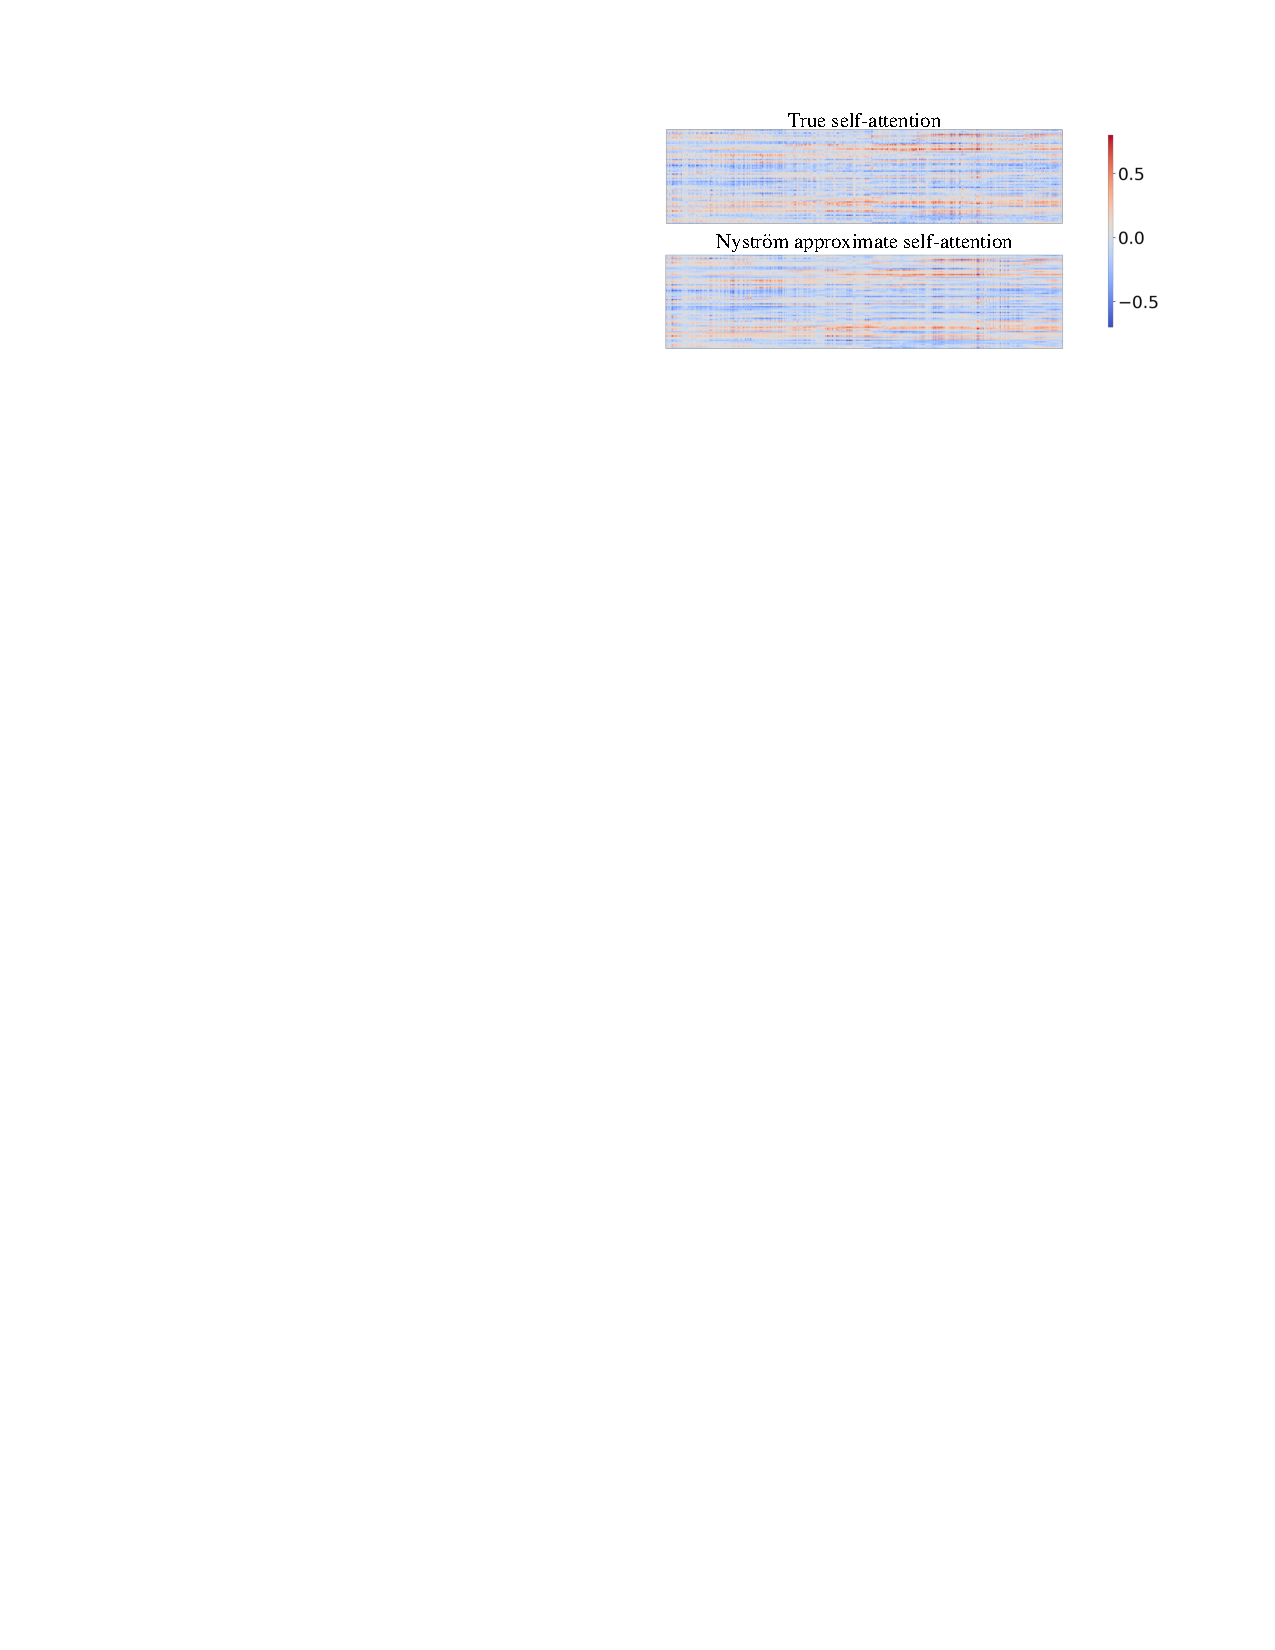
\includegraphics{nystrom_example.pdf}
        \caption[\nystr{} Attention Example]{Anecdotal comparision of the true attention and Nystr\"om approximation. Reprinted from \citep{nystrom}.}
        \label{fig:nystrom_example}
\end{figure}

The authors note that thanks to the theoretical results from \citep{nystr-2017} and \citep{linformer}, even a small number of landmarks suffices to provide a good approximation.
The first paper states that the error of the Nystr\"om approximation decreases with the matrix's rank.
In the second paper, the authors suggest that the attention mechanism produces low-rank matrices.  

\subsection{Encoder Utilization in Document Retrieval}

We have, so far, introduced the encoder model, but we have yet to describe how to use it in document retrieval. We can look at the neural-model-generated encodings in a way similar to the traditional approaches.

Traditional approaches result in a sparse representation of the knowledge base with the feature dimensionality equal to the corpus's vocabulary size (the vocabulary can also contain n-grams or character n-grams if it is advantageous).
Therefore, it can be considered a weighting scheme, assigning "importance" to each word present in the document. 
% Neural approaches in this paper produce a dense representation -- a fixed-size vector of real numbers, inherently hard to interpret.

Neural approaches in this paper generate a fixed-length real-valued vector representation for both the query and all the documents in the knowledge base.
The dense representation is inherently hard to interpret, and the meaning can be derived only from the relative position of different documents' representations (vectors).
Hence the $f(q,d)$ score from Equation \ref{eq:formal_descr_dr} is the distance between the vector representations of $q$ and $d$.
The distance metric used may be cosine similarity, dot product, or fast approximation such as FAISS \citep{faiss}.
This approach allows us to preprocess the whole knowledge base, allowing us to compute only the query representation during runtime.
The disadvantage is that we do not utilize the attention mechanism to consider each query-document relation individually and, today less relevant problem, the need for additional space to store the precomputed representation.

Neural models can also be used directly as the scoring function as in Equation \ref{eq:formal_descr_dr} and use the document-query pair $(d,q)$ as their input (the cross-attention model).
This can, according to \citet{two-tower}, lead to better performance. However, since the query is provided at runtime, the evaluation cannot be precomputed and has to run for every document each time we enter a new query.
Because of that, and because of the large number of documents in the knowledge base, this approach is unfit for real-world application.

There exists a hybrid approach capable of utilizing the cross-attention model. 
It runs the model on a small subset of the corpus, typically pre-selected by a non-neural model.
The model only reranks the gathered sentences.
Our colleague \citet{dedkova} provides a detailed look into the use of such methods in Czech document retrieval.

% i did not mention it
%As mentioned above, when dealing with natural language processing, we can approach the task in two different ways, both described in detail by \cite{two-tower}. 

%USED ABOVE
%The first is to have the document-query pair $(d,q)$ on the input of the neural model (cross-attention model).
%One of the benefits is the direct usage of the neural model on the downstream tasks, possibly granting better performance.

%USED ABOVE
%The second approach generates a fixed-length real-valued vector representation for both the query and all the documents in the knowledge base.
%Then the $f(q,d)$ score is the distance between $q$'s and $d$'s representation.
%The distance metric used may be cosine similarity, dot product, or some approximation such as FAISS \citep{faiss}.

%BLAH SOUNDS TOO SIMPLE The second approach is to preprocess the whole database of documents by the model and then using some metric for choosing the documents related to the query based on the computed representation.
%The obvious advantage is the offline preprocessing and thus improved performance during inference.
%Only the unseen query has to be processed by the neural model followed by computing the metric between the documents' representation and the query representation.
%This approach grants significant speedup compared to computing the score for every query-document pair. 

%USED ABOVE
%We will be using the second approach since the number of documents in our knowledge base renders the cross-attention paradigm computationally unfit for real-world application.
% TODO vymazat, 
%In order to solve the document retrieval task, we will focus on finding an appropriate function $f$.
%In this thesis, that means a function suitable for long documents.

\subsubsection{Generating Representations}

Generating the dense representations, also called embeddings since we project the input into a vector space with a specific dimension, is, in general, a well-studied area of research. We restrict ourselves to neural methods described in Section \ref{sec:neural_approaches}. 

There are multiple ways to generate the input's embedding from the model-processed tokens.
Sentence-BERT \citep{sbert} adds a pooling layer, either \texttt{MAX} or \texttt{MEAN}, and fine-tunes the model using two different approaches, depending on the task.
For regression tasks, TODO.
They compare their method against averaging all the output tokens' representations, selecting the out representation of special input token \texttt{[CLS]} situated at the front of the input, and against averaging input tokens' GloVe \citep{glove} word vectors.
The authors note that if the fine-tuning step is not performed, the BERT model provides little to no improvement to averaging input tokens' word vectors.

The authors of \citep{two-tower} proposed a different approach, designed directly for document retrieval, in their case, over Wikipedia articles. 
They apply a fully-connected linear layer to the \texttt{[CLS]} token's representation and also pre-train the BERT model on three additional document retrieval tasks:
\begin{itemize}
        \item \textbf{Inverse Cloze Task (ICT)} - Training the model to embed sentences close to the paragraph from which they were selected. The selected sentences are omitted from the paragraph in the training step.
        \item \textbf{Body First Selection (BFS)} - Training the model to embed sentences close to the paragraphs in the same article. The sentences are selected in such a manner to reasonably expect this task to succeed. In the case of training on Wikipedia, the sentences are selected from the first paragraph (summary).
        \item \textbf{Wiki Link Prediction (WLP)} - Training the model to embed sentences close to Wikipedia articles from which there exists a hyperlink to the article of the sentence.
\end{itemize}
The authors reported significant improvements compared to using only MLM for the pre-training phase.
% USED ABOVE They use the model's final representation of the special input token \verb{[CLS]}, situated at the front of the input, as the representation of the whole input. 

\subsection{Czech Language}

TODO
%The introduced BERT-based models are seldom trained on Czech data.

\subsection{Distillation}

TODO
\chapter{Datasets}
\label{chap:data}

% TODO was it really mentioned
As mentioned, the primary dataset, usage-wise and inspiration-wise, was the FEVER dataset \citep{fever}.
Deriving from \cite{fever} methods, we \citep{ullrich} were able to create our own FEVER-like database using Czech News Agency's infobank.

\section{FEVER Dataset}

\textbf{F}act \textbf{E}xtraction and \textbf{Ver}ification \citep{fever} dataset is a large-scale dataset based on Wikipedia articles.
The dataset was created by extracting sentences (claims) from the English Wikipedia articles and classifying them by human annotators as Supported, Refuted, or NotEnoughInfo.
If the claim is verifiable (Supported, Refuted), then the evidence, either single or multiple paragraphs or even articles proving or disproving the claim, is also recorded.
The complete FEVER contains 185,445 annotated claims generated using 50,000 popular articles.

The creation consisted of two steps. The sentences were first manually extracted from popular Wikipedia articles.
Only the first paragraphs, usually containing the summary, were used for this step. 
Then, to create a more diverse set of claims, the annotators had the option of producing new claims by mutating the existing ones in various ways (generalizing, specification, entity substitution, non-trivial negating, and rephrasing).
The negation used has to be non-trivial because simple negative words and phrases like ``no'' and ``it is not true that'' can be leveraged by the later steps of the fact-checking pipeline to immediately classify claims as Refuted instead of trying to understand the text.

More complex claims were created by providing related Wikipedia articles (articles hyperlinked from the original article) as another source of information while mutating the claim.

In the second step - annotation - the annotators were asked to label the generated claims and provide suggested evidence when needed.
The whole process was streamlined to not spend longer than five minutes on a single claim throughout all stages.

The quality of the dataset was thoroughly tested in the paper.
We have, however, noticed an unaddressed issue described in Section \ref{subsec:data_leakage}.
One of the methods for improving the dataset was annotating the generated claim by multiple people to reduce mislabeling.

\subsection{FEVER CS}

For use in baseline training and pre-training, we localized the original FEVER dataset into the Czech language. 
The localization consisted of translating the original claims using a translation service and mapping the English Wikipedia knowledge base used by FEVER to available Czech Wikipedia articles while removing claims with missing Czech evidence.
The process is in-depth described by \citet[Chapter 3]{ullrich}.

\begin{table}[h!]
    \centering
    \begin{tabular}{c || c c c || c c c}
        \multirow{2}{0.8cm}{Split} & \multicolumn{3}{c||}{FEVER CS} & \multicolumn{3}{c}{FEVER EN} \\
        & Supported & Refuted & NEI & Supported & Refuted & NEI\\
        \hline
        train & 53,542 & 18,149 & 35,639 & 80,035 & 29,775 & 35,639\\
        dev & 3,333 & 3,333 & 3,333 & 6,666 & 6,666 & 6,666 \\
        test & 3,333 & 3,333 & 3,333 & 6,666 & 6,666 & 6,666
    \end{tabular}
\caption[Fever CS Label Distribution]{Label distribution of the resulting FEVER CS.}
\end{table}

Because of the large-scale usage of machine translation without the means for robust evaluation and the lack of one-to-one correspondence between Czech and English Wikipedia articles, this dataset serves only as a baseline to verify the robustness of our models on a larger scale, primarily for the document retrieval part of the pipeline.

\begin{figure}[h!]
    \begin{framed}
    \begin{verbatim}
    {
      "id": 120449,
      "verifiable": "VERIFIABLE",
      "label": "SUPPORTS",
      "claim": "Venuše se nazývá 'sesterskou planetou' Země.",
      "evidence": [
        [
          [
            141476,
            156671,
            "Venuše (planeta)",
            8,
            "Venus"
          ]
        ]
      ],
      "claim_en": "Venus is called the \"sister planet\" of Earth."
    }\end{verbatim}
    \vspace{-0.4cm}
    \end{framed}
    \caption[FEVER CS Data Example]{FEVER CS data example, containing one evidence set refering to the Venus Wikipedia page.}
    \label{fig:fevercs_example}
\end{figure}

\section{\CTK}
% nomenclature

The basis for this dataset is the collection of Czech news articles provided in collaboration with the Czech News Agency. 
Inspired by \cite{fever} and \cite{danish_fever}, our colleague \cite{ullrich} created a Czech version of the claim extracting and labeling software tool\footnote{available at \url{https://fcheck.fel.cvut.cz/}} running over the ČTK infobank's articles. 
%TODO insert image
It was designed to be used by layman annotators, who were students of our partner - the Faculty of Social Sciences at Charles University.

\begin{table}[h!]
\centering
\begin{tabular}{c || c c c}
    Split & Supported & Refuted & NotEnoughInfo \\
    \hline
    train & 1132 & 519 & 473 \\
    dev & 100 & 100 & 100 \\
    test & 200 & 200 & 200
\end{tabular}
\caption[\CTK{} Dataset Label Distribution]{Label distribution of the resulting \CTK{} v2.1 dataset.}
\end{table}

The dataset creation consisted of two harvests. 
After reviewing the results of the first one, we were able to rewrite instructions in the tool to guide the annotators to create higher-quality claims and labels with fewer conflicts.
The second harvest concluded with $\approx$ 3,500 labeled claims, with more than half being labeled two or more times. %TODO cite webpage
As of writing, this figure is not final as the dataset needs to be manually cleaned and have conflicts resolved. 

\begin{figure}[h!]
    \begin{framed}
    \begin{verbatim}
    {
      "id": 2143,
      "label": "REFUTES",
      "claim": "Kocianovo kvarteto nikdy nezískalo žádné ocenění.",
      "evidence": [
        [
          "T200706010229101_1"
        ]
      ],
      "source": "T200706010229101_1"
    }\end{verbatim}
    \vspace{-0.4cm}
    \end{framed}
    \caption[\CTK{} Dataset Example]{\CTK{} data example, containing one evidence set refering to the first paragraph of the \CTK{} infobank article with the id \texttt{T200706010229101}.}
    \label{fig:ctk_example}
\end{figure}

\begin{figure}[h!]
    \begin{framed}
        Paříž/Praha 2. června (ČTK) - Za vynikající kompletní nahrávku kvartetů Paula Hindemitha pro francouzskou firmu Harmonia Mundi obdrželo 3. června 1997 české Kocianovo kvarteto Velkou cenu francouzské Akademie Charlese Crose.
    \end{framed}
    \caption[\CTK{} Infobank Example]{\CTK{} infobank entry corresponging to the evidence id in Figure \ref{fig:ctk_example}.}
\end{figure}

\begin{figure}[h!]
  %\makebox[\textwidth][c]{{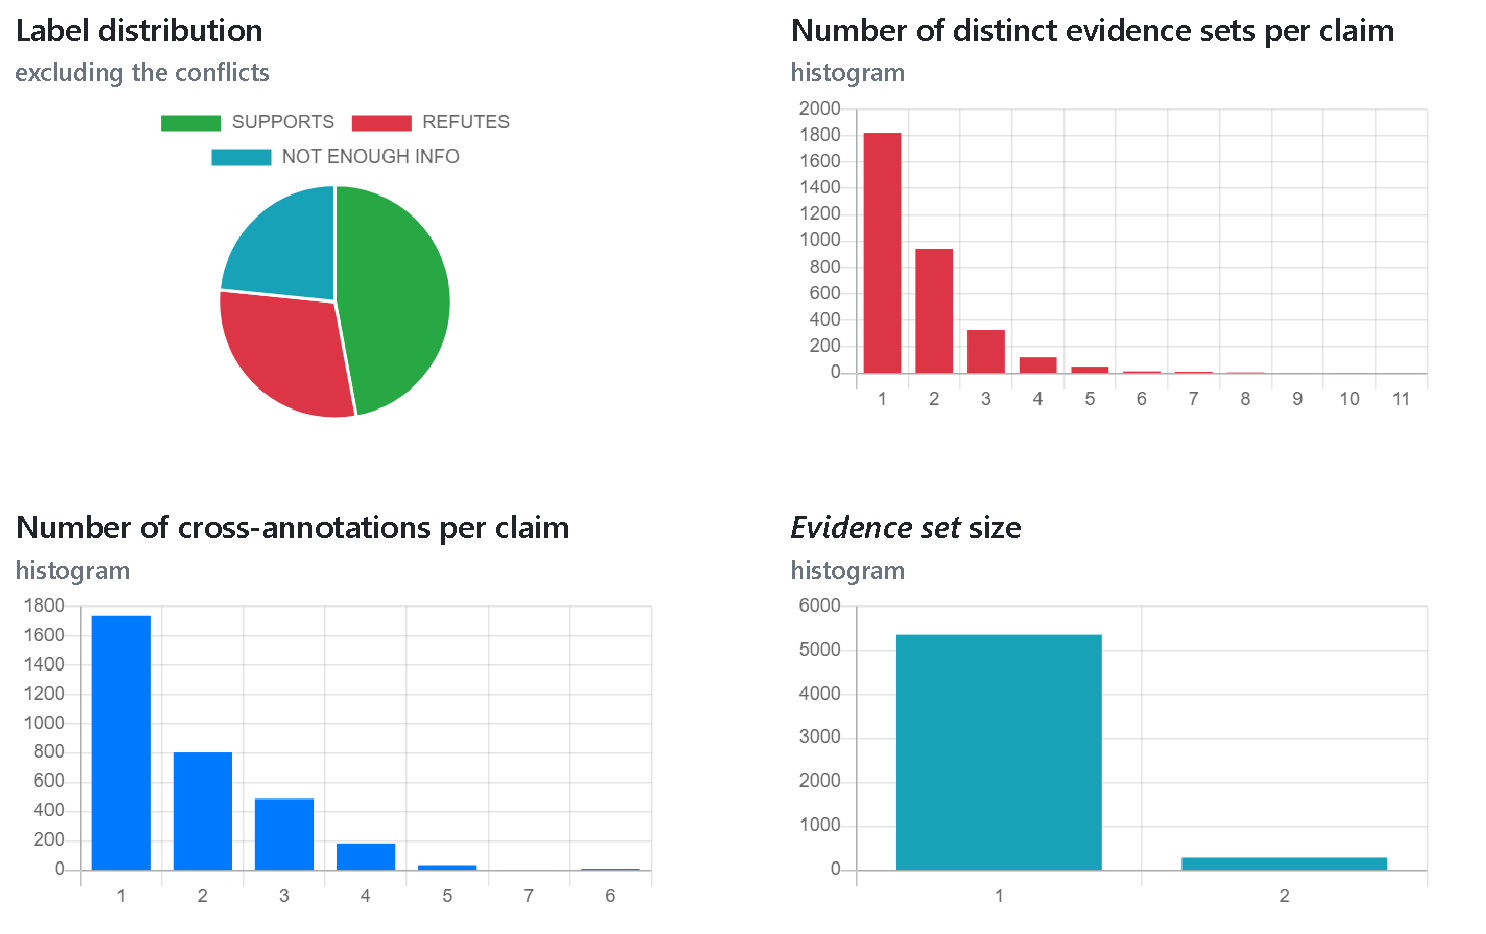
\includegraphics[width=16cm]{dashboard.pdf}}}
  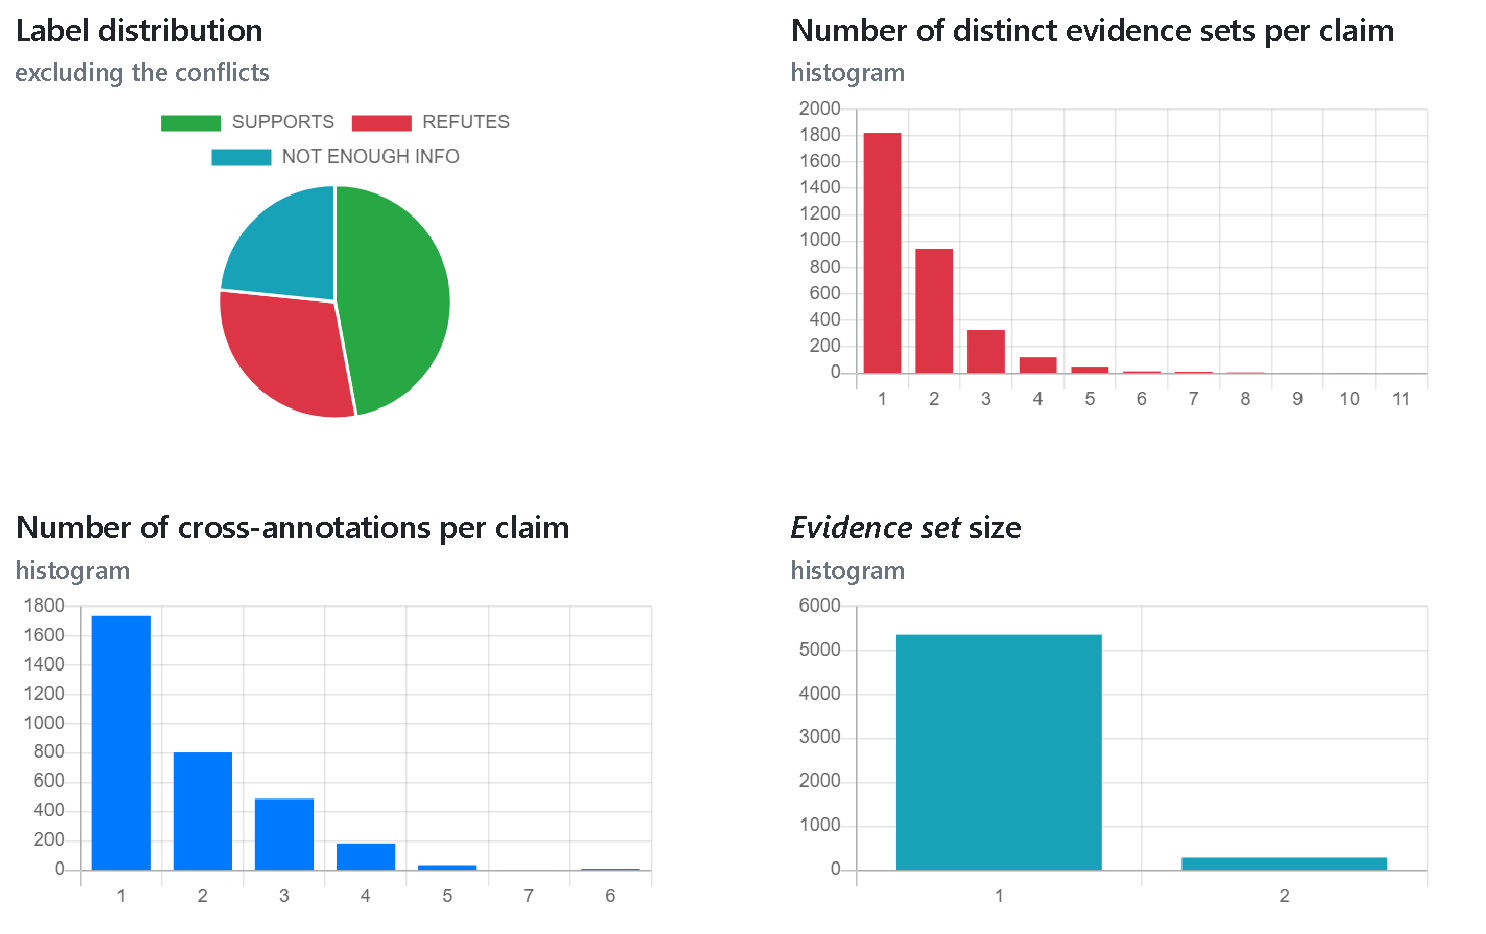
\includegraphics[width=\textwidth]{dashboard.pdf}
  \caption[Visualizations of Properties of the Collected Dataset]{Visualizations of various properties of the collected \CTK{} dataset. Figure reprinted from \citet{ullrich}.}
  \label{fig:dashboard}
\end{figure}

\section{Data Quality}

The claim mutation in FEVER and \CTK{} datasets can be a source of unintentional cues, which the model can use to "guess" the label without understanding the claim.
For example, \citet{fever} pointed out that their annotators had difficulties negating the claims beyond trivial negations.

\citet{rypar} conducted a series of evaluations on the \CTK{} and FEVER CS datasets using dataset-weighted cue information (DCI), and cue productivity and coverage \citep{niven-probing}, inspired by \citet{derczynski-etal-2020-maintaining}.
The results concluded that the original FEVER dataset contained simple negative clues, which were also present in FEVER CS, although with limited impact only. No significant bias was confirmed, but the current size of the \CTK{} dataset allows for thematic clusters which impact the dataset more than they should. 

\subsection{Data Leakage}
\label{subsec:data_leakage}

As pointed out by \citet{ullrich}, the original FEVER dataset CONTAINS a not addressed quality -- at least 80 \% of verifiable dev claims share an evidence-set document with some train claim. The effects of this "leakage" are unknown and call for further research.
\chapter{Proposed Solutions}

\section{Baselines}

As the traditional baseline, we have decided to use BM25, as proposed by \citet{weak-baselines}.
We use the Pyserini\footnote{\url{https://github.com/castorini/pyserini/}} python toolkit for information retrieval \citep{pyserini} -- a python interface for the Anserini\footnote{\url{https://github.com/castorini/Anserini}} library \citep{anserini1, anserini2}, originally implemented in Java, building on the Lucene\footnote{\url{https://lucene.apache.org/}} library.
The Pyserini library is a highly optimized library implementing multiple search algorithms.
We also compare our results with the results achieved by \citet{rypar}, who researched document retrieval for documents up to one paragraph long ($\approx$ 230 tokens), using mBERT and ColBERT \citep{colbert} models.

\section{Neural Models}

Following the discussion in Section \ref{sec:data_length}, we have chosen the input length of the model to be 2048. 
Given the resource-intensity of the task, we have chosen to test the \nystr{} model 

\section{Evaluation Metrics}

Document retrieval is best evaluated when dealing with evidence sets by the model's ability to match the evidence set with retrieved documents.
By the retrieved documents, we mean the sequence of $k$ documents from the knowledge base with the highest scores.
We can match the evidence set in a variety of ways, motivating multiple measures of performance:
\begin{itemize}
    \item \textbf{Precision} - We try to ``fit within'' the evidence set with retrieved documents.
    \item \textbf{Recall} - We try to ``cover'' the evidence set.
    \item \textbf{F1} - The harmonic mean of precision and recall. 
    \item \textbf{Mean Reciprocal Rank (MRR)} \citep{mrr} - We try to retrieve the relevant documents at the first positions. 
\end{itemize}
The specific formulas are: 
\begin{equation}
    \text{precision} = \frac{|\{\text{evidence documents}\}\cap\{\text{retrieved documents}\}|}{|\{\text{retrieved documents}\}|}\ ,
\end{equation}
\begin{equation}
    \text{recall} = \frac{|\{\text{evidence documents}\}\cap\{\text{retrieved documents}\}|}{|\{\text{evidence documents}\}|}\ ,
\end{equation}
\begin{equation}
    \text{F1} = 
    %\frac{2}{\frac{1}{\text{precision}}+\frac{1}{\text{recall}}} =
    \frac{2\cdot\text{precision}\cdot\text{recall}}{\text{precision}+\text{recall}}\ ,
\end{equation}
\begin{equation}
    \text{MRR} = \frac{1}{|Q|}\sum_{i=1}^{|Q|}{\frac{1}{\text{rank}_i}}\ ,
\end{equation}
where $Q$ is a sequence of queries and $\text{rank}_i$ is the rank of the first relevant document retrieved for the query $q_i$.

The most relevant metrics for us will be recall and MRR, since we aim to provide all the necessary knowledge ideally as the top results. 
Since precision and recall depend on the number $k$ of retrieved documents, we evaluate the models with varying $k$ and denote each evaluation with the suffix $\text{@}k$.
\chapter{Experiments}

\section{BM25}

We used grid search for $k_1 \in [0.2,2.0]$, $b\in[0.1,1.0]$ with the step size of $0.1$, over training data.
Only the entries labeled supported and refuted were used since only such entries provide evidence.
We performed fine-tuning over whole training splits for both \CTK{} and FEVER CS datasets.
% For the \CTK{} dataset, we performed the fine-tuning over the whole training split, while for the FEVER CS dataset, we randomly selected 10,000 verifiable claims from the training set.
The resulting parameters were chosen according to the best recall achieved on the training data, calculated by summing up the difference between the best-achieved recall$@k$ and the configuration's recall$@k$.
The monitored levels of the parameter $k$ were 1, 5, 10, 25, 50, 100, and 500. 
The resulting values of the hyperparameters are displayed in Table \ref{tab:bm25_finetune}. 
We note that the difference between the selected values and neighboring values was marginal (see Table \ref{tab:bm25_sets}). 
%\begin{table}[!htb]
    %\centering
    %\begin{subtable}[t]{.47\textwidth}
        %\centering
        %\begin{tabular}{lrr}
            %datset & $k_1$ & $b$ \\
            %\midrule
            %\CTK{} & 1.0 & 0.5 \\
            %FEVER CS & 1.4 & 0.3
        %\end{tabular}
        %%\caption[BM25 Fine-tuned Parameters]{Fine-tuned parameters for BM25.}
        %%\label{tab:bm25_finetune}
    %\end{subtable}
    %\hfill
    %\begin{subtable}[t]{.47\textwidth}
        %\centering
        %\begin{tabular}{lcc}
            %datset & $k_1$ & $b$ \\
            %\midrule
            %\CTK{} & [0.9, 1.1] & [0.4, 0.5] \\
            %FEVER CS & [1.3, 1.5] & [0.3, 0.4]
        %\end{tabular}
        %%\caption[BM25 Promising Parameter Sets]{Neighbourhoods of parameter values with best results on the training sets.}
        %%\label{tab:bm25_sets}
    %\end{subtable}
    %\caption[BM25 Parameter Selection]{Results of BM25 fine-tuning. \textbf{Left}: The selected fine-tuned parameters. \textbf{Right}: Neighbourhoods of parameter values with the best performance.}
%\end{table}
\begin{table}[!htb]
    \centering
    \begin{minipage}[t]{.47\textwidth}    
        \centering
        \begin{tabular}{lrr}
            datset & $k_1$ & $b$ \\
            \midrule
            \CTK{} & 1.0 & 0.5 \\
            FEVER CS & 1.4 & 0.3
        \end{tabular}
        \caption[BM25 Fine-tuned Parameters]{Fine-tuned parameters for BM25.}
        \label{tab:bm25_finetune}
    \end{minipage}
    \hfill
    \begin{minipage}[t]{.47\textwidth}
        \centering
        \begin{tabular}{lcc}
            datset & $k_1$ & $b$ \\
            \midrule
            \CTK{} & [0.9, 1.1] & [0.4, 0.5] \\
            FEVER CS & [1.3, 1.5] & [0.3, 0.4]
        \end{tabular}
        \caption[BM25 Promising Parameter Sets]{Neighbourhoods of parameter values with the best performance.}
        \label{tab:bm25_sets}
    \end{minipage}
\end{table}

\section{Results}
\subsection{\CTK}
\subsection{FEVER CS}

\section{Discussion}

\chapter*{Conclusion}
\addcontentsline{toc}{chapter}{Conclusion}

We introduced the problem of fact-checking and described modern approaches to the problem.
We explained the motivation for studying the topic and proposed using new neural models to help with automatic fact-checking.
Our research team created the first fact-checking dataset in the Czech language \citep{ullrich} and explored different models' architectures capable of good performance.
Inspired by the FEVER pipeline \citep{fever} (see Figure \ref{fig:pipeline}), we split the problem into two distinct tasks -- document retrieval and natural language inference.

In this thesis, we deal with the document retrieval task.
We first defined the task formally and then introduced well-established traditional techniques for the task.
Then followed a brief description of the progress from RNN-based language models to transformers \citep{attention-is-all-you-need} and BERT \citep{bert}.
Since the BERT model as described in \citep{bert} and as adopted across the research field perform best only for inputs up to 512 tokens, we were forced to work over paragraphs instead of the whole documents. 
Our colleagues \citep{rypar} and \citep{dedkova} studied this type of document retrieval.

This thesis explored whether we could improve retrieval performance by utilizing whole articles. 
We provided a summary of currently available papers regarding transformer language models supporting long inputs, namely Longformer, BigBird, Reformer, Linformer, Performer, and \nystr{}.
Since no pre-trained models for the Czech language were available, we either trained them from scratch or utilized the student-teacher method \citep{student-teacher} described in Section \ref{subsec:distillation}.
Lastly, we compared the traditional, short-input, and long-input approaches in the document retrieval task and analyzed the results.

The resulting models turned out not to outperform classic BERT with paragraph-level splitting, but TODO.

\subsubsection{Future Work}

As time progresses, automatic fact-checking will be needed more and more.
With the joint effort across the machine learning research field, we hope to train better TODO.
We wish to continue improving the created \CTK{} dataset and to now focus on the natural language inference task of the fact-checking pipeline. 

%%% Bibliography
%%% Bibliography (literature used as a source)
%%%
%%% We employ bibTeX to construct the bibliography. It processes
%%% citations in the text (e.g., the \cite{...} macro) and looks up
%%% relevant entries in the bibliography.bib file.
%%%
%%% The \bibliographystyle command selects, which style will be used
%%% for references from the text. The argument in curly brackets is
%%% the name of the corresponding style file (*.bst). Both styles
%%% mentioned in this template are included in LaTeX distributions.

\bibliographystyle{plainnat}    %% Author (year)
% \bibliographystyle{unsrt}     %% [number]

\renewcommand{\bibname}{Bibliography}

%%% Generate the bibliography. Beware that if you cited no works,
%%% the empty list will be omitted completely.

\bibliography{bibliography}

%%% If case you prefer to write the bibliography manually (without bibTeX),
%%% you can use the following. Please follow the ISO 690 standard and
%%% citation conventions of your field of research.

% \begin{thebibliography}{99}
%
% \bibitem{lamport94}
%   {\sc Lamport,} Leslie.
%   \emph{\LaTeX: A Document Preparation System}.
%   2nd edition.
%   Massachusetts: Addison Wesley, 1994.
%   ISBN 0-201-52983-1.
%
% \end{thebibliography}


%%% Abbreviations used in the thesis, if any, including their explanation
%%% In mathematical theses, it could be better to move the list of abbreviations to the beginning of the thesis.
%\chapwithtoc{List of Abbreviations}
\chapter*{Appendix A - Acronyms}
\addcontentsline{toc}{chapter}{Appendices}
\begin{description}
    \itemsep0em
    \item[BERT] Bidirectional Encoder Representations from Transformers
    \item[FEVER] Fact Extraction and Verification 
    \item[GPT-3] Generative Pre-trained Transformer 3
    \item[ČVUT] České Vysoké Učení Technické (Czech Technical University in Prague)
    \item[\CTK{}] Česká Tisková Kancelář (Czech News Agency)
    \item[NEI] Not Enough Info
    \item[TREC] Text Retrieval Conference
    \item[NNLM] Neural Networks 
    \item[TFIDF] Term Frequency - Inverse Document Frequency
    \item[BM25] Best Match 25
    \item[TF] Term Frequency
    \item[IDF] Inverse Document Frequency
    \item[BOW] Bag of Words
    \item[RNN] Recurent Neural Networks
    \item[Seq2Seq] Sequence to Sequence
    \item[SOTA] State of The Art
    \item[NER] Named Entity Recognition
    \item[NLI] Natural Language Inference
    \item[QA] Question Answering
    \item[ICT] Inverse Cloze Task
    \item[BFS] Body First Selection
    \item[WLP] Wiki Link Prediction 
    \item[FAISS] Facebook AI Similarity Search
    \item[GloVe] Global vectors for word representation
    \item[SBERT] Sentence-BERT
    \item[RoBERTa] Robustly optimized BERT 
    \item[XLM-R] XL Multilingual RoBERTa
    \item[SGD] Stochastic Gradient Descend
    \item[LSH] Locality-sensitive Hashing
    \item[CNN] Convolutional Neural Networks
    \item[RevNet] Reversible Residual Networks
    \item[iid] Independent and Identically Distributed
    \item[DCI] Dataset-weighted Cue Information
    \item[mBERT] multilingual BERT
    \item[SNLI] The Stanford Natural Language Inference (SNLI) Corpus
    \item[MRR] Mean Reciprocal Rank
\end{description}
\chapter*{LRA Model Comparison}
\addcontentsline{toc}{chapter}{A2 \nystr{} LRA Comparison}

The authors of the \nystr{} model \citep{nystrom} published the following comparision between the \nystr{}, Performer \citep{performer}, Linformer \citep{linformer}, and Reformer \citep{reformer} models:

\begin{figure}[!htb]
    \centering
    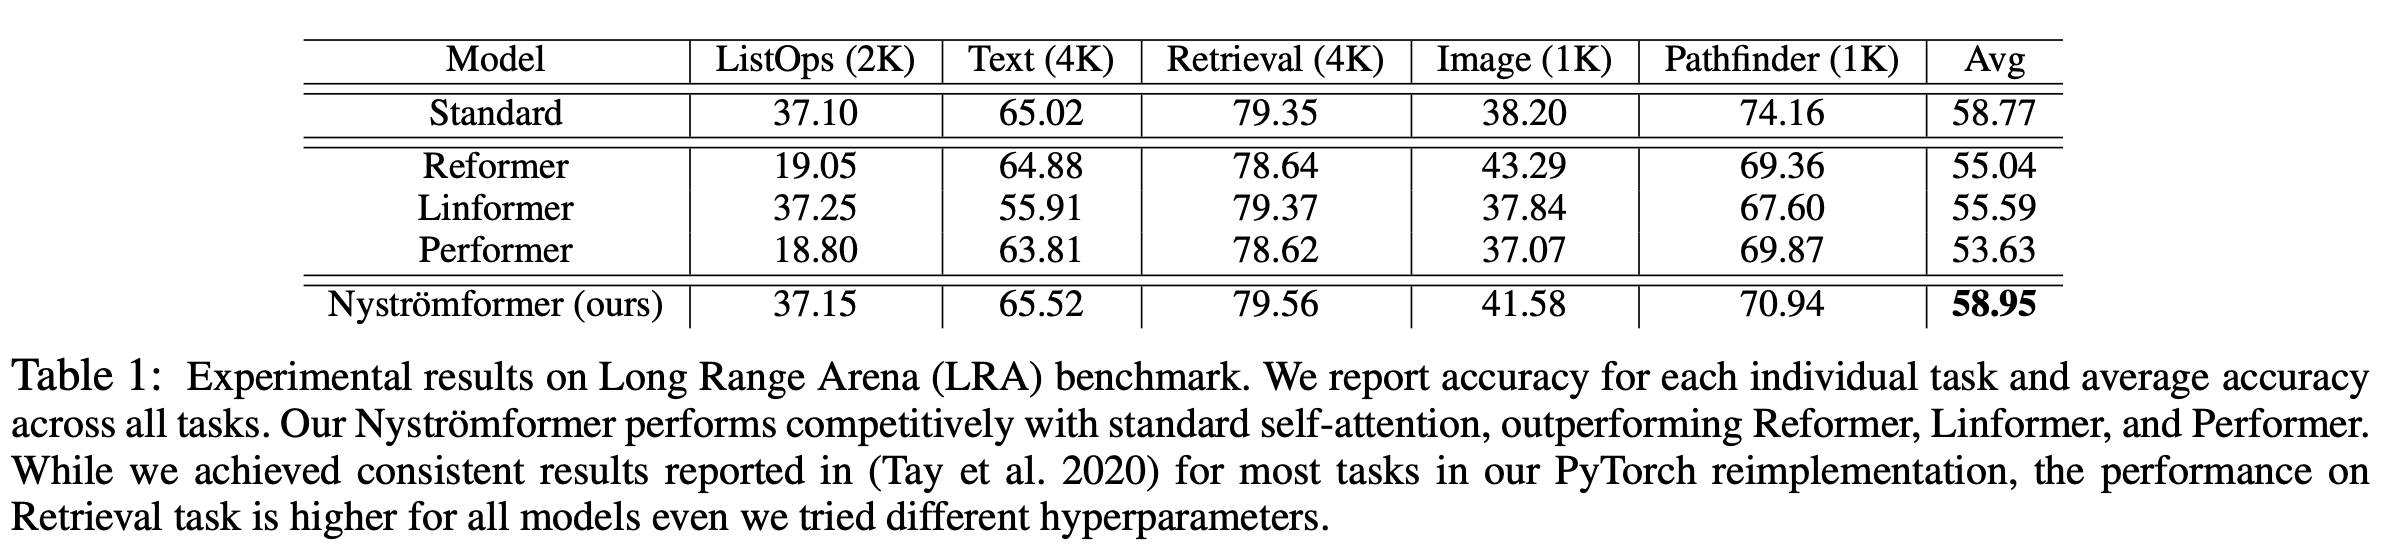
\includegraphics[width=\linewidth]{nystr_LRA.png}
    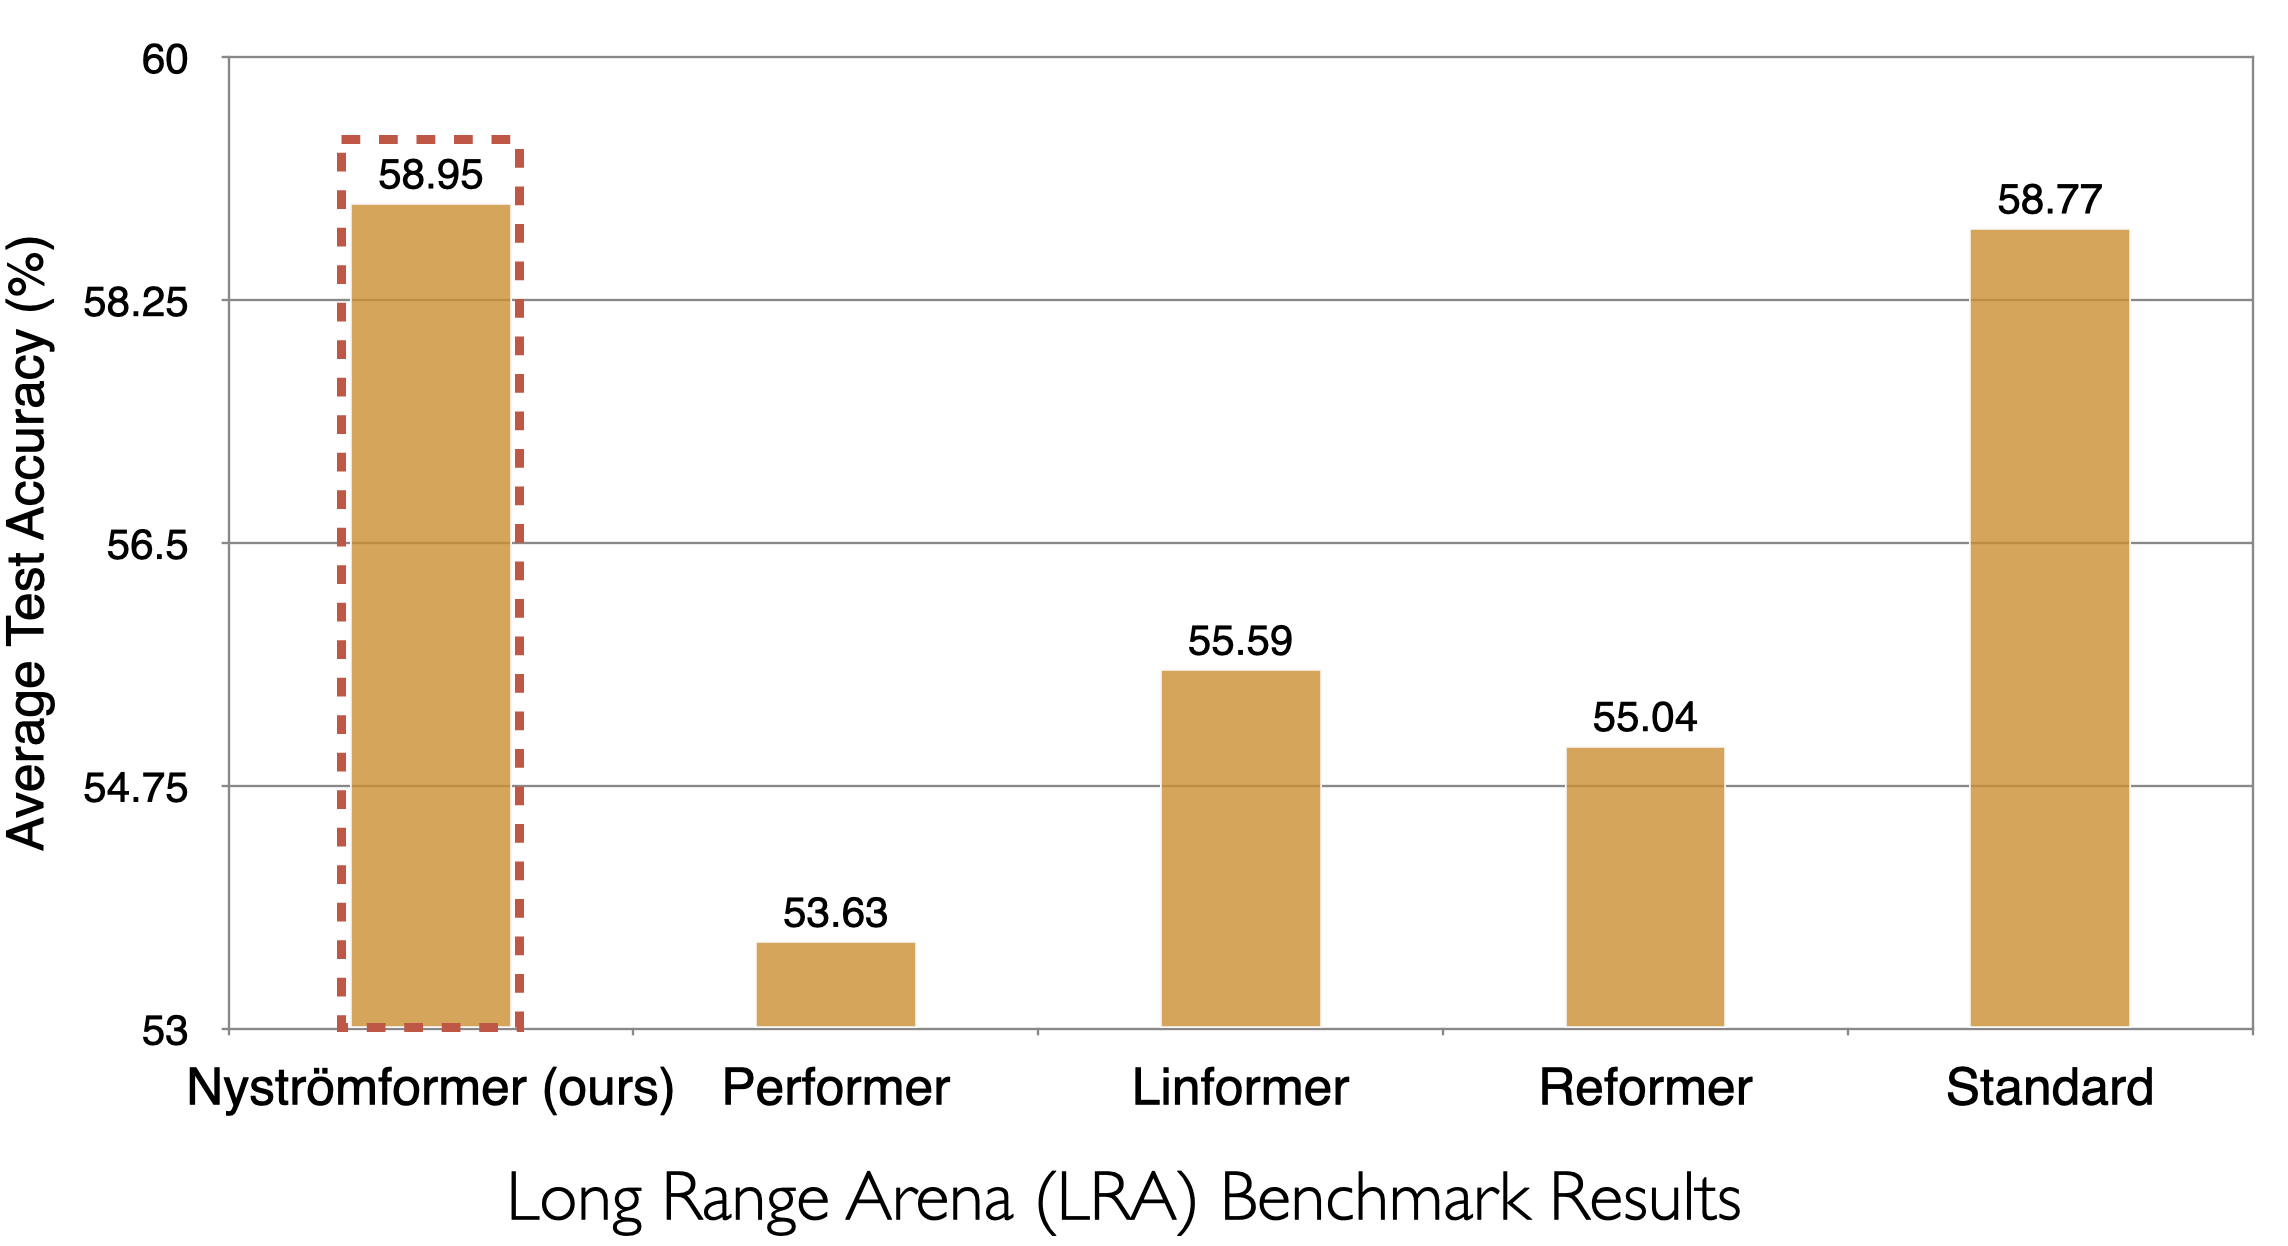
\includegraphics[width=\textwidth]{nystr_avg_LRA.png}
    \caption*{The upper figure reprinted from \citep{nystrom}, the bottom figure reprinted from the attached repository\footnote{\url{https://github.com/mlpen/Nystromformer/}}.}
\end{figure}
\chapter*{Appendix C - Code Repository}
%\addcontentsline{toc}{chapter}{A2 \nystr{} LRA Comparison}

The code used in this thesis is avalilable at \url{https://gitlab.fel.cvut.cz/factchecking/master-thesis-code}. It contains multiple ad hoc jupyter notebooks, which were comfortable to work with using remote access to the cluster. Distinct subtasks reside in their own respective directories.

\openright
\end{document}